\graphicspath{ {img/BR/} }
\chapter[Bandwidth Reservation as a Coexistence Strategy in Opportunistic Spectrum Access Environments][Bandwidth Reservation in OSA]{Bandwidth Reservation as a Coexistence Strategy in Opportunistic Spectrum Access Environments}\label{BR_chap}
\section{Introduction}\label{sec:Introduction}
Because of the sensing and transmission problem described in the previous chapter, consequence of the hardware limitations of cognitive devices, there is always some probability of PU and SU transmission overlap and therefore some level of interference at the PUs.
In fact, OSA relies on the idea that it makes sense to minimally reduce the QoS of the primary network (PN) if it would result in a much higher spectrum efficiency \cite{ref:Pawelczak2009}.
Previous research efforts have been mainly focused on designing OSA for the best SU performance at a desired level of PU QoS protection \cite{ref:Domenico2012}. In contrast, the PN point of view has not received enough attention, let alone the consideration of the PN as an active agent collaborating in OSA. And, as we expalined in the introduction, the consent of the spectrum owners is vital to the implementation of DSA mechanisms. 

\subsection{Motivation}
The question addressed in this chapter is: is it worth for the PN to reserve part of its spectrum for easing OSA to a secondary network (SN)? The reserved channels will only be used by the PUs if the non-reserved ones are occupied by other PU transmissions. 
Intuitively, it seems to be beneficial for the SUs, since it eases finding spectrum opportunities and assures that the free channels are adjacent, simplifying the SU's transmission hardware.
The incentives for the PN are not so clear. On the one hand it might avoid collisions with SU transmissions, resulting in less interference at PU receivers, but on the other hand it would reduce the amount of channels available to the PN resource allocation algorithm. In a PN exploiting the channels with best instantaneous propagation conditions, the reservation scheme would reduce the achievable rate.
Determining when the positive aspects compensate the negative ones is not a trivial question and depends on several characteristics of the system: the PU traffic, the SU traffic, the configuration of OSA parameters, the transmission parameters, etc.

The situation considered is not only theoretical. There are scenarios where it would be a feasible coexistence framework. For example, in areas where the regulators force OSA in a licensed spectrum band, it would be an affordable way for the licensed operator to minimize the harmful effects of SU activity. Or if a spectrum owner decides to grant access to certain spectrum bands in exchange for a pre-established flat-rate fee for SUs. This solution could be an alternative to the more complex automatic spectrum trading mechanisms in the literature \cite{ref:Gao2011}, \cite{ref:Yu2010}, and more feasible in the early stages of cognitive radio deployment, not requiring the introduction of new protocols, interfaces, etc, as spectrum trading does \cite{ref:Yang2011}. With the scheme described in this chapter, the licensed operator maintains the reserved band free of PU activity with a high probability and the cognitive users assure, by means of their sensing capabilities and short transmissions periods, a small collision probability and a low interference level with PU communications.
 
\subsection{Related Work}\label{sec:RelatedWork}
In many networking technologies we can find examples of mechanisms for exploiting spare network resources. For example, in circuit switched networks, it is usual to use protection provisioned capacity to accommodate low-priority traffic in failure-free conditions \cite{ref:Vasseur2004}.
In wireless networks, channel reservation schemes were applied to reduce the dropping probability of handover calls \cite{ref:Ramjee1996}, \cite{ref:Vazquez2006}. 
Although the bandwidth reservation idea studied in this paper is conceptually similar to those classic schemes, its application in opportunistic spectrum access environments is completely different in many technical aspects: interference and propagation issues, the sensing of PU activity, the variability of the channel gain, the effect of BR on PU Shannon capacity, among others. Therefore, new research challenges have to be addressed.

Despite the intense research effort conducted on cognitive radio so far, the issue of bandwidth reservation for OSA and its impact on SU and PN performance has not been yet addressed in detail.
The term channel reservation in cognitive radio environments is used in \cite{ref:Zhu2007} and later works like \cite{ref:Martinez2009}, \cite{ref:Ahmed2009} and \cite{ref:Lai2011} to refer to a mechanism by which some of the channels not used by the PN are kept free of SU traffic by the secondary network (SN) itself. These ``reserved channels'' are used by the SN to accommodate ongoing SU transmissions that, forced by PUs, have to leave their initially occupied channels. In that case, the reservation is performed by the SN at the cost of an increased SU blocking probability. That idea is indeed an adaptation of the classic handoff channel reservation scheme to the cognitive environment.

To the best of our knowledge, only one work \cite{ref:Tang2006} has considered reserving part of the spectrum so that PUs only occupy the second part when the first one is congested.
While \cite{ref:Tang2006} assumed that the PN was completely unaffected by the introduction of a SN and by the reservation scheme, we base our study on the fact that, in real systems, both SU activity and bandwidth reservation do actually have an impact on PU performance. Therefore, we present the idea not as a way to minimize the SN blocking probability, but as a strategy to simultaneously improve PU and SU capacities in a coexistence scenario. Moreover we develop a detailed, realistic model comprising hardware constraints, multichannel OSA, propagation effects and interference.

In the framework of spectrum trading, a recent work \cite{ref:Wu2012} proposed a system in which the PN reserves a set of channels for dynamic spectrum auction. This work follows the concept of spectrum pooling, where secondary users temporarily rent from a pool of spectrum resources from primary users \cite{ref:Biglieri2012}. This approach requires the implementation of new protocols to support the required PU-SU signaling and makes the spectrum sensing no longer needed. It is therefore essentially different to the opportunistic access framework of our proposal.

There have been extensive research efforts involving OSA for low-complexity, hardware constrained devices \cite{ref:Park2011}, \cite{ref:Li2012} as well as multichannel access \cite{ref:Jeon2012}, \cite{ref:Xu2012_eff}. 
Several works like \cite{ref:Jia2008_HC}, \cite{ref:Kim2008}, \cite{ref:Gabran2011} and \cite{ref:Cheng2011} consider both characteristics simultaneously. As in \cite{ref:Jia2008_HC} we consider that, because of the SU's hardware limitations, sensing can only be conducted within a small portion of the spectrum (channels) and requires a non-negligible time (scanning delay). Our model also includes imperfect sensing, bayesian estimation and the effects of PU interference on SU achievable bit rate.  


Because we are interested in evaluating the capacity of the licensed network, the resource allocation scheme of the PN has to be capable of exploiting all the available bandwidth, implying full channel awareness. This is the goal of OFDM scheduling mechanisms \cite{ref:Sadr2009}. Our model considers one simple but effective mechanism described in \cite{ref:Sadr2009} and \cite{ref:Rhee2000}.
In works centered on cognitive MAC, the PN is usually characterized by collision probability \cite{ref:Gabran2011}, \cite{ref:Jung2012}, \cite{ref:Zhao2007_dec} and \cite{ref:Huang2009}, and less frequently by overlapping time \cite{ref:Huang2008_opp}.
However, for more general evaluations of PN and SN coexistence, interference level at PU receivers or PN Shannon capacity is preferred \cite{ref:Sun2012}. In OFDM related works, performance is usually evaluated in terms of capacity or achievable rate \cite{ref:Sadr2009}, \cite{ref:Rhee2000}, as we do in this work. The novelty in our analysis is obtaining closed-form analytical expressions for the capacity under OSA interference, with and without BR.

\subsection{Our Contribution}
The main contribution of this chapter is to develop a detailed framework for evaluating the impact of the bandwidth reservation scheme on PU and SU performance.
Based on the numerical results obtained, we discuss under which conditions and why it is recommendable or not to implement a PN channel reservation scheme for OSA and how to configure it.
As we explain in Section \ref{sec:System}, the SUs are characterized by hardware-limited radio, imperfect spectrum sensing, multichannel access, and a Maximum A Posteriory (MAP) estimator of the PU activity in the scanned channels. Section \ref{sec:System} also describes the PN resource allocation model.
In Section \ref{sec:Model} we derive the transition probabilities of the Markov model for the PU-SU channel occupation process.
By means of the Markov-reward model detailed in Section \ref{sec:Reward}, we evaluate the joint PU and SU performance in terms of expected total capacity, interference power and collision probability.

\section{System Description}\label{sec:System}
\subsection{Licensed Network}
The system under study consists of two overlay wireless networks. The licensed one operates with centralized access coordinated by an access node (AN). 
As in previous works (e.g. \cite{ref:Zhao2007_dec}, \cite{ref:Kim2008},\cite{ref:Gelabert2011}, \cite{ref:Jiao2012}, \cite{ref:Tang2009}), PU traffic is assumed to follow a Poisson model: PU inter-arrival time and channel holding time are exponential random variables with rates $\lambda_{p}$ and $\mu_{p}$ respectively.

We are evaluating the impact of the spectrum reservation scheme on the capacity of the licensed network. Therefore we consider that the AN's resource allocation mechanism exploits all the available bandwidth independently of the number of PUs connected.
We only consider resource allocation in the downlink bandwidth, were the OSA operates.

\subsubsection{Radio Resource Allocation of the Licensed Network} 
The downlink spectrum consists of $N$ channels or subcarriers, each one with a bandwidth of $W$ Hz. At each time-slot, each one of the $n_{p}$ PUs in the system is assigned one of the $N$ channels and part of the total transmission power $p_{PU}$ of the AN.
At time-slot $t$, the wireless link between the $j$-th PU and the AN is associated to $N$ channel gains, one for each channel. The channels are assumed to present a constant gain over the bandwidth $W$ and over the duration $\tau$ of the time-slot, and change over consecutive time-slots due to fading effects (block fading model, \cite{ref:Goldsmith2005}).
A perfect channel state information is assumed, so that the AN knows all the channel gains at each time-slot.
The objective of the resource management algorithm is to assign one channel to each PU and to allocate the power $p_{PU}$ among the $n_{p}$ assigned channels, at each time-slot, such that the total PU capacity is maximized.
A well known strategy to attain this objective is to use a flat transmit power spectral density (PSD) \cite{ref:Rhee2000}, i.e. all the assigned subcarriers are allocated the same power ($p_{PU}/n_{p}$). This simplifies the problem to a subcarrier allocation problem which is solved by allocating the best available subcarrier to the PU with the least achieved rate, and then allocating the best subcarrier among the $N-1$ remaining ones to the PU with the second least rate, and so on. This strategy is shown to assure fairness among users and to achieve 96\% of the optimum capacity (\cite{ref:Rhee2000}, \cite{ref:Sadr2009}).

\subsubsection{Bandwidth Reservation for OSA} 
The bandwidth reservation (BR) mechanism considered implies that the AN reserves $m$ adjacent downlink channels for OSA, and the remaining $N-m$ channels are assigned to the $n_{p}$ PUs following the subcarrier allocation strategy described, whenever $n_{p}\leq N-m$. In case $n_{p}>N-m$, part of the $m$ reserved channels (concretely $n_{p}+m-N$) are assigned to PU transmissions, such that the $n_{p}$ channels used for PUs remain adjacent among them. Summarizing, the spectrum available for PU downlink transmission contains $\text{max}\left(n_{p},N-m\right)$ adjacent channels. Figure \ref{BR_fig_allocation} shows an example of the BR mechanism studied.

\begin{figure}[ht]
\centering
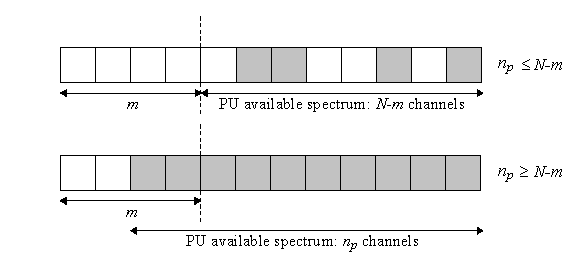
\includegraphics[scale=0.9]{channelReservation.eps}
\caption[]{Channel reservation scheme in the licensed spectrum. Greyed-out channels are occupied by PUs.}\label{BR_fig_allocation}
\end{figure}

\subsection{Secondary Network}\label{secondarynetwork}
The unlicensed or secondary network operates in a decentralized, ad-hoc fashion. 
Communication is always performed between pairs of SUs (\textit{cognitive pairs}) consisting of one sender and one receiver.
Every SU is assumed to be under the coverage area of the same licensed access node, thus the objective is to transmit data using one or several of the $N$ licensed channels causing the less possible degradation to PU communications. The SU access follows the interweave paradigm \cite{ref:Biglieri2012}, avoiding simultaneous transmissions with PUs.

In line with the low complexity, hardware limited approach of previous works (e.g. \cite{ref:Pawelczak2009} as \cite{ref:Jia2008_HC}, \cite{ref:Li2012}), the MAC protocol of the SUs is similar to the hardware-constrained MAC described in \cite{ref:Jia2008_HC}.
Summarizing, HC-MAC comprises three consecutive phases: \textit{contention}, \textit{sensing} and \textit{transmission}.
The contention procedure allows a pair of SUs (sender and receiver) to reserve the use of the spectrum in a certain area avoiding collisions with other SU transmissions.
Then, the cognitive pair starts to sense the spectrum in fixed-duration sensing slots to detect PU activity on each channel. 
As in \cite{ref:Jia2008_HC}, the hardware limitations of the SUs are:
(1) Each SU is equipped with a single radio that can either transmit or receive, but not at the same time.
(2) When scanning the spectrum to detect PU activity, an SU can only sense one narrowband channel during each sensing slot.
(3) Once a cognitive pair decides to start a transmission, it can use up to $n_{s,\text{max}}$ noncontiguous channels simultaneously. 

For the sake of completeness, we consider imperfect sensing, which can result in false positive or false negative PU activity detection. The false positive and false negative probabilities, $p_{f}$ and $p_{n}$, are computed for an energy level detector, using the formulas presented in \cite{ref:Pawelczak2009} and the references therein. The parameters involved are the sensing slot duration $s$, the channel bandwidth $W$, the observed signal to noise ratio, and the detection threshold $\theta$.

\begin{figure}[ht]
\centering
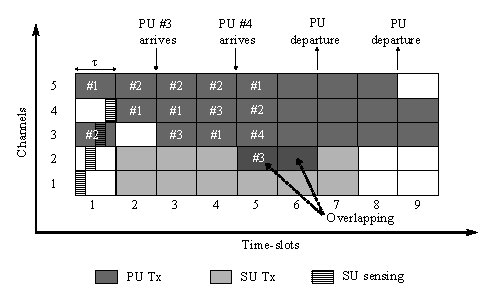
\includegraphics[scale=1]{slots.eps}
\caption[]{Sensing and access phases in OSA. The SU scans $\Delta=4$ channels, and detects $a=3$ available channels. In this case, the SU is leaving 1 free channel. This happens when the safety margin is $k=1$ or when the SU channel occupation limit is $n_{s,\text{max}}=2$. During the SU transmission, two PUs arrive, causing transmission overlap in channel 2 during time-slots 5 and 6. The numbers $\#n$ identify the PU to which the channel is assigned at each time-slot.}\label{BR_fig_slots}
\end{figure}

During the sensing phase, the SU scans $\Delta$ channels.
Because this phase lasts one time-slot, the sensing slot duration is $s=\tau/\Delta$.
If BR is used, the SU only transmits in the available channels found in the $m$ reserved channels. If not, the SU can transmit in the free channels found in $\Delta$.  
In both cases the SU can use up to $n_{s,\text{max}}$ and, depending on the configuration, it may have to leave $k$ free channels, as a safety margin.
Figure \ref{BR_fig_slots} shows an example of the sensing and access phases.
Table \ref{BR_table_parameters} summarizes the most relevant parameters of the model. Some of them have been already presented in this section and others are explained in Sections \ref{sec:Model} and \ref{sec:Reward}. We also include a brief list of the abbreviations used.

\begin{table}
\begin{tabular}{ll} \hline
\textbf{Abbreviation} & \textbf{Definition}\\\hline
$PU$ & Primary User\\
$PN$ & Primary Network\\
$AN$ & Access Node\\
$SU$ & Secondary User\\
$OSA$ & Opportunistic Spectrum Access\\
$BR$ & Bandwidth Reservation\\
$MAC$ & Medium Access Control\\
$MAP$ & Maximum A Posteriori\\
$PSD$ & Power Spectral Density\\\hline
\textbf{Notation} & \textbf{Definition}\\\hline
$W$ & channel bandwidth\\
$\tau$ & duration of the time-slots\\
$\Delta$ & number of scanned channes\\
$k$ & safety margin\\
$n_{s,\text{max}}$ & maximum channels for SU Tx\\
$m$ & reserved channels in BR\\
$\lambda_{p}$ & PU's arrival rate\\
$\mu_{p}$ & PU's service rate\\
$\pi_{i}$ & probability of PU activity in channel $i$\\
$p_{s}$ & probability of SU arrival\\
$q_{s}$ & probability of SU departure\\
$\rho_{s}$ & SU traffic intensity\\
$T_{s}$ & average duration of an SU transmission\\
$n_{s}$	& number of SU's in the system\\
$n_{p}$	& number of PU's in the system\\
$C_{j_N}\left(n_{p}\right)$ & $j$-th PU capacity without interference\\
${C}_{N}\left(n_{p}\right)$ & PU capacity without interference\\
$C^{I}_{j,N}\left(n_{p},n_{s}\right)$ & $j$-th PU capacity with interference\\
$C^{\text{nbr}}_{N}\left(n_{p},n_{s}\right)$ & per state PN capacity without BR\\
$C^{\text{br}}_{N}\left(n_{p},n_{s}\right)$ & per state PN capacity with BR\\
$\bar{R}^{\text{nbr}}_{PU}$ & normalized PN capacity without BR\\
$\bar{R}^{\text{br}}_{PU}$ & normalized PN capacity with BR\\
$C'^{\text{nbr}}_{N}\left(n_{p},n_{s}\right)$ & per state SU capacity without BR\\
$C'^{\text{br}}_{N}\left(n_{p},n_{s}\right)$ & per state SU capacity with BR\\
$\bar{R}^{\text{nbr}}_{SU}$ & normalized SU capacity without BR\\
$\bar{R}^{\text{br}}_{SU}$ & normalized SU capacity with BR\\\hline
\end{tabular}
\centering
\caption{Summary of the most relevant parameters of the model}
\label{BR_table_parameters}
\end{table}

\section{Spectrum Occupation Model}\label{sec:Model}
\subsection{Spectrum Occupation Process}
Upon a PU arrival, the incoming PU is admitted in if there are available channels, and remains in the system for a random time, exponentially distributed with rate $\mu_{p}$. If $n_{p}=N$, incoming PUs are rejected (blocking event).
Because the system operates in a time-slot basis, we translate the PU channel occupation process into a set of probabilities $P_{p}(j|i)$, for $i,j \in \left\{0,1,\ldots,N\right\}$, defined as the probability that $n_{p}=j$ in time-slot $t+1$, given that $n_{p}=i$ in time-slot $t$. 
These $P_{p}(j|i)$ are the elements of the $\left(N+1\right)\times\left(N+1\right)$ transition probability matrix $\mathbf{T}$. The stationary distribution $\bar{\pi} = \left(\pi_{0},\pi_{1},\dots,\pi_{N}\right)$ is obtained from the equilibrium equations $\bar{\pi} = \bar{\pi}\mathbf{T}$, $\left\|\bar{\pi}\right\|_{1} = \sum_{i=1}^{m}\pi_{i}=1$.
This process is essentially a discrete-time $M/M/N/N$ queue (in Kendall's notation), with blocking probability equal to $\pi_{N}$.

Let us now consider the PU process in conjunction with OSA. At each time slot, the probability that an SU attempts to access the spectrum is $p_{s}$.
An incoming SU scans the spectrum and then starts an SU transmission period using the detected free channels up to a maximum $n_{s,\text{max}}$. Considering $n_{s,\text{max}}$ as a safety limit, the OSA MAC assures that no other SU attempts to access the spectrum if another SU is using it. The model could be generalized to accommodate several concurrent SU transmissions, although, for evaluation purposes, it would be equivalent to increase $n_{s,\text{max}}$ in the presented model.  
For an incoming SU, we define the opportunistic access probability, $O\left(n'_{s},n_{p}\right)$, as the probability that the SU occupies $n'_{s}$ channels in time-slot $t+1$ given that there are $n_{p}$ PUs using the spectrum in time-slot $t$.
The duration of an SU transmission period is, in average, $T_{s}$, after which the SU leaves the spectrum. The termination probability of an SU transmission is $q_{s}=1/T_{s}$.
As a result, considering the SU access process in absence of PU activity, the probability that the spectrum contains an SU transmission is given by $\rho_{s}=p_{s}/(p_{s}+q_{s})$, which we will refer to as the SU traffic intensity. Note that the actual probability of SU activity in the system will be lower than $\rho_{s}$, in general, because, the spectrum sensing may not always find spectrum opportunities.


This model describes the spectrum occupation process as a Markov chain, $Z_{t}$ with a state space consisting of a set of pairs, $\left(n_{s},n_{p}\right)$, such that $n_{s} \in \left\{0,1,\dots,n_{s,\text{max}}\right\}$ and $n_{p} \in \left\{0,1,\dots,N\right\}$. 
The transition probabilities from state $Z_{t}=\left(n_{s},n_{p}\right)$ to $Z_{t+1}=\left(n'_{s},n'_{p}\right)$ are given by
\begin{equation}\label{TransitionProbabilities}
P\left(n'_{s},n'_{p}|n_{s},n_{p}\right) = 
\begin{cases}
p_{s}O_{s}\left(n'_{s},n_{p}\right)P_{p}\left(n'_{p}|n_{p}\right)&\mbox{if } n_{s}=0,\:n'_{s}\neq0\\
q_{s}\left(n_{s}\right)P_{p}\left(n'_{p}|n_{p}\right)&\mbox{if } n_{s}\neq0,\:n'_{s} = 0\\
\left(\left(1-p_{s}\right) + p_{s}O_{s}\left(0,n_{p}\right)\right)P_{p}\left(n'_{p}|n_{p}\right)&\mbox{if } n_{s}=n'_{s}=0\\
\left(1-q_{s}\right)P_{p}\left(n'_{p}|n_{p}\right)&\mbox{if } n_{s}=n'_{s}\neq0\\
0&\mbox{otherwise}\\
\end{cases}
\end{equation}
% \begin{equation}\label{TransitionProbabilities}
% \begin{array}{l}
% P\left(n'_{s},n'_{p}|n_{s},n_{p}\right) = \\
% \begin{cases}
% p_{s}O_{s}\left(n'_{s},n_{p}\right)P_{p}\left(n'_{p}|n_{p}\right)&\mbox{if } n_{s}=0,\:n'_{s}\neq0\\
% q_{s}\left(n_{s}\right)P_{p}\left(n'_{p}|n_{p}\right)&\mbox{if } n_{s}\neq0,\:n'_{s} = 0\\
% \left(\left(1-p_{s}\right) + p_{s}O_{s}\left(0,n_{p}\right)\right)P_{p}\left(n'_{p}|n_{p}\right)&\mbox{if } n_{s}=n'_{s}=0\\
% \left(1-q_{s}\right)P_{p}\left(n'_{p}|n_{p}\right)&\mbox{if } n_{s}=n'_{s}\neq0\\
% 0&\mbox{otherwise}\\
% \end{cases}
% \end{array}
% \end{equation}
The following subsections develop the derivation of $O_{s}\left(n'_{s},n_{p}\right)$ for each spectrum reservation policy.

\subsection{SU Spectrum Sensing}
After the sensing phase, the SU generates an estimate $\hat{h}$ of the number $h$ of occupied channels in the scanned spectrum.
The estimation is based upon the sensing outcome, $\mathbf{x} = \left(x_{1},\dots,x_{\Delta}\right)$, where $x_{i} = 1$ if the SU detected PU activity in channel $i$ and $x_{i} = 0$ otherwise. We consider that the SU obtains $\hat{h}$ by a Maximum A Posteriori (MAP) estimation, $\hat{h}~=~\text{argmax }_{h} P\left(h|\mathbf{x}\right)$, which, applying Bayes' rule is equivalent to $\hat{h}~=~\text{argmax }_{h} P\left(h\right)P\left(\mathbf{x}|h\right)$ (see \cite{ref:Bertsekas2008}),
where $P\left(h\right)$ and $P\left(\mathbf{x}|h\right)$ can be obtained from the PU traffic and sensing error models, and depend on the spectrum reservation policy.

\subsubsection{Without Spectrum Reservation}
The conditional distribution $P\left(\mathbf{x}|h\right)$ of each outcome can be obtained as follows.
For each $\mathbf{x}$ the number of positive detections is $\left\|\mathbf{x}\right\|_{1}=\sum_{i=1}^{\Delta}x_{i}$.
For a given $h$, the number of false positives $f_{\text{p}}$ in $\mathbf{x}$ ranges from $f_{\text{p,min}}=\left(\left\|\mathbf{x}\right\|_{1}-h\right)^{+}$ to $f_{\text{p,max}}=\text{min}\left(\left\|\mathbf{x}\right\|_{1},\Delta-h\right)$.
For each $f_{\text{p}}$, the following equations provide the number of correct positives $c_{\text{p}}$, false negatives $f_{\text{n}}$ and correct negatives $c_{\text{n}}$ in $\mathbf{x}$:
\begin{equation}
\begin{array}{lcl}
c_{\text{p}} & = & \left\|\mathbf{x}\right\|_{1} - f_{\text{p}}\\
f_{\text{n}} & = & h-\left(\left\|\mathbf{x}\right\|_{1} - f_{\text{p}}\right)\\
c_{\text{n}} & = & \Delta - \left\|\mathbf{x}\right\|_{1} - f_{\text{n}}
\end{array}
\end{equation}
Then, adding the probabilities of all the possible $f_{\text{p}}$ values yields 
\begin{equation}\label{Pxh}
P\left(\mathbf{x}|h\right) = \displaystyle\sum^{f_{\text{p,max}}}_{f_{\text{p}}=f_{\text{p,min}}}
{\Delta-h \choose f_{\text{p}}}{h \choose c_{\text{p}}} p_{n}^{f_{\text{n}}}\left(1-p_{n}\right)^{c_{\text{p}}}p_{f}^{f_{\text{p}}}\left(1-p_{f}\right)^{c_{\text{n}}}
\end{equation}

When $j$ PUs are randomly allocated over $N$ channels, the number $h$ of PUs in the $\Delta$ scanned channels is a hypergeometrical random variable denoted by $P_{\text{H}}\left(h;N,j,\Delta\right)$. 
To obtain the distribution $P(h)$ we apply the law of total probability on every possible value of $h$:
\begin{equation}\label{Ph}
P\left(h\right) =
\begin{cases}
\sum_{j=h}^{N-\Delta+h}\pi_{j}P_{\text{H}}\left(h;N,j,\Delta\right)&,\mbox{if }h>0\\
\sum_{j=0}^{N-\Delta}\pi_{j}P_{\text{H}}\left(h;N,j,\Delta\right)&,\mbox{if }h=0
\end{cases}
\end{equation}

\subsubsection{With Spectrum Reservation}
The SU is assumed to scan, at least, the $m$ reserved channels. Therefore, $\mathbf{x}=\left(\mathbf{x}_{m}, \mathbf{x}_{\Delta-m}\right)$, where $\mathbf{x}_{m}$ is the observation obtained in the first $m$ scanned channels and $\mathbf{x}_{\Delta-m}$ is the observation in the $\Delta-m$ channels scanned in the non-reserved spectrum. Similarly, $h=h_{m}+h_{\Delta-m}$, where $h_{m}$ and $h_{\Delta-m}$ are the PUs in the reserved and non-reserved channels respectively. The probabilities $P\left(\mathbf{x}_{\Delta-m}|h_{\Delta-m}\right)$ and $P\left(h_{\Delta-m}\right)$ are computed using (\ref{Pxh}) and (\ref{Ph}) respectively, for $\Delta-m$ scanned channels. In the reserved spectrum, the PUs occupy contiguous channels, therefore, for a given $h_{m}$, we can obtain $f_{\text{p}}$, $c_{\text{n}}$, $f_{\text{n}}$, and $c_{\text{p}}$ in $\mathbf{x}_{m}$ as follows
\begin{equation}
\begin{array}{lcl}
f_{\text{p}} & = & \sum_{j=h_{m}+1}^{m}x_{j}\\
c_{\text{n}} & = & m-h_{m}-\sum_{j=h_{m}+1}^{m}x_{j}\\
f_{\text{n}} & = & h_{m}-\sum_{j=1}^{h_{m}}x_{j}\\
c_{\text{p}} & = & \sum_{j=1}^{h_{m}}x_{j}
\end{array}
\end{equation}
and the conditional probability $P\left(\mathbf{x}_{m}|h_{m}\right)$ is given by
\begin{equation}
P\left(\mathbf{x}_{m}|h_{m}\right) = p_{n}^{f_{\text{n}}}\left(1-p_{n}\right)^{c_{\text{p}}}p_{f}^{f_{\text{p}}}\left(1-p_{f}\right)^{c_{\text{n}}}
\end{equation}
The distribution $P(h_{m})$ is directly obtained from $\bar{\pi}$:
\begin{equation}
P\left(h_{m}\right) =
\begin{cases}
\pi_{N-m+h}&,\mbox{if }h_{m}>0\\
\sum_{j=0}^{N-m}\pi_{j}&,\mbox{if }h_{m}=0
\end{cases}
\end{equation}
\subsection{SU Spectrum Access}
Let $D_{\Delta}\left(a,h\right)$ denote the probability of finding a number $a$ of available channels given that, during the sensing phase, $h$ out of the $\Delta$ scanned channels are occupied by PU transmissions. 
In order to compute $D_{\Delta}\left(a,h\right)$ let us define $X_{\hat{h}}$ as the set of possible values of $\mathbf{x}$ for which the outcome of the MAP estimator equals $\hat{h}$: $X_{\hat{h}} = \left\{\mathbf{x}|\hat{h} = \underset{h}{\text{argmax }} P\left(h\right)P\left(\mathbf{x}|h\right)\right\}$.

Finding $a$ free channels implies detecting PU activity in $\hat{h}=\Delta-a$, therefore
 $D_{\Delta}\left(a,h\right)$ is given by
\begin{equation}
\begin{array}{lcl}
D_{\Delta}\left(a,h\right) & = & P(\hat{h}|h)\\
& = & \sum_{\mathbf{x}\in X_{\hat{h}=\Delta-a}}P\left(\mathbf{x}|h\right)
\end{array}
\end{equation}  
Let us consider the no BR and the BR cases separately for the computation of $O_{s}\left(n'_{s},n_{p}\right)$ .
\subsubsection{Without Spectrum Reservation}
The probability that, in any time slot, $h$ channels out of $\Delta$ scanned channels are used by PUs, when there are $n_{p}$ PUs in the spectrum, is hypergeometrical. Therefore
\begin{equation}\label{Os1}
O_{s}\left(n'_{s},n_{p}\right) = 
\begin{cases} \displaystyle\sum_{h=h_{\text{min}}}^{h_{\text{max}}}D_{\Delta}\left(n'_{s}+k,h\right)P_{\text{H}}\left(h;N,n_{p},\Delta\right)&\mbox{if } n'_{s}<n_{s,\text{max}}\\
\displaystyle\sum_{a=n'_{s}+k}^{\Delta}\displaystyle\sum_{h=h_{\text{min}}}^{h_{\text{max}}}D_{\Delta}\left(a,h\right)P_{\text{H}}\left(h;N,n_{p},\Delta\right)&\mbox{if } n'_{s}=n_{s,\text{max}}
\end{cases}
\end{equation} 
where $h_{\text{min}} = \left(\Delta+n_{p}-N\right)^{+}$ and $h_{\text{max}} = \mbox{min}\left(\Delta,n_{p}\right)$ are the minimum and maximum number of PUs within $\Delta$.
\subsubsection{With Spectrum Reservation}
In this case, an incoming SU occupies $n'_{s}$ channels, always within the $m$ reserved ones. Therefore, the SU detects $a_{m}=\text{min}\left(m,n'_{s}+k\right)$ in the $m$ reserved channels and $a_{\Delta-m}=\left(n'_{s}+k-m\right)^{+}$ in the no reserved ones. For $n_{p}>N-m$, $h_{m}=n_{p}+m-N$ and $h_{\Delta-m} = \Delta-m$, therefore 
\begin{equation}\label{Os2}
O_{s}\left(n'_{s},n_{p}\right) = D_{m}\left(a_{m},h_{m}\right)D_{\Delta-m}\left(a_{\Delta-m},h_{\Delta-m}\right)
\end{equation}
For $n_{p}\leq N-m$, $h_{m}=0$ and each value of $h_{\Delta-m}$ has a hypergeometric probability $P_{\text{H}}\left(h_{\Delta-m};N,n_{p},\Delta-m\right)$. Multiplying (\ref{Os1}) by the $D_{m}\left(a_{m},h_{m}\right)$ term, we can obtain $O_{s}\left(n'_{s},n_{p}\right)$. In case $n'_{s}=n_{s,\text{max}}$, the outer summation is done over $a_{\Delta-m}=\Delta-m,\ldots,n'_{s}+k-m$.

\section{Markov Reward Model for PU and SU Capacities}\label{sec:Reward}
In this section we construct a Markov reward model to estimate the achievable transmission rate for PUs and SUs. Such a model requires the definition of a reward function $R\left(n_{s},n_{p}\right)$ providing the Shannon capacity at each state. The objective is to obtain the expected average reward defined as
\begin{equation}\label{MarkovReward1}
\bar{R} = \underset{T\rightarrow\infty}{\text{lim }}\frac{1}{T}\displaystyle\sum_{t = 0}^{T}R\left(Z_{t}\right)
\end{equation}
For an ergodic, finite-state Markov chain, and provided that $\left|R\left(n_{s},n_{p}\right)\right|$ is bounded for every $\left(n_{s},n_{p}\right)$, the total expected average reward $\bar{R}$ is
\begin{equation}\label{MarkovReward2}
\bar{R} = \displaystyle\sum_{n_{p} = 0}^{N}\sum_{n_{s} = 0}^{m-k}R\left(n_{s},n_{p}\right)P(n_{s},n_{p})
\end{equation}
where $P(n_{s},n_{p})$ are the steady state probabilities of the Markov process defined by (\ref{TransitionProbabilities}).

\subsection{Propagation model}
Before deriving the expressions for PU and SU capacities with and without BR, we have to establish the models for the pathloss and fading effects on the transmitted signals. Let $p_{PU}$ denote the total available transmission power at the PU Tx (AN) for the whole spectrum. The power transmitted in each channel, when there are $n_{p}$ PUs, is $p_{p}=p_{PU}/n_{p}$ (flat transmit PSD). The average received power at a PU terminal, after considering the path loss, is referred to as $p_{pp}$. Similarly, $p_{SU}$, $p_{s}$, and $p_{ss}$, are the total power at the SU Tx, the SU power in one channel, and the average SU received power in one channel, respectively. For interference computations, we use $p_{sp}$ to refer to the average SU power received at a PU Rx location and $p_{ps}$ for the PU power at an SU Rx location. Figure \ref{BR_fig_interference} shows a diagram with the transmission and interference powers between PUs and SUs.

\begin{figure}[ht]
\centering
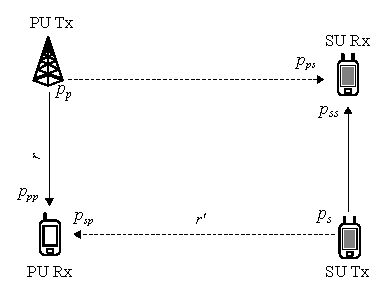
\includegraphics[scale=1]{interference.eps}
\caption[]{Diagram of the interference between PUs and SUs.}\label{BR_fig_interference}
\end{figure} 

For path loss estimation, we consider a common empirical method known as piecewise linear model (see \cite{ref:Goldsmith2005}). In this model, for a given distance $r$ between the Tx and the Rx, the average received power is approximately equal to $p_{pp}=p_{p}Kg(r)$, where $K$ is a constant depending on the antenna gains, and $g(r)$ is given by
\begin{equation}
g(r) =  
\begin{cases}
1 &\mbox{if }r\leq 1\\
r^{-n_{1}} &\mbox{if }1<r\leq r_{c}\\
r_{c}^{-n_{1}}\left(\frac{r}{r_{c}}\right)^{-n_{2}} &\mbox{if }r> r_{c}\\
\end{cases}
\end{equation}
The parameters $n_{1}$, $n_{2}$ and $r_{c}$ are empirically determined depending on the propagation environment. Typical values are around $n_{1}=2$, $n_{2}=4$, and $r_{c}=100$ (that we use in our model).
The same $g(r)$ is also used for SU signals.

The instantaneous received power changes in consecutive time-slots due to multipath fading effects, and is characterized by a probability density function (\textit{pdf}).
In particular, assuming that the fading amplitude follows a Rayleigh distribution, the received power has the following \textit{pdf}, $f(p)=e^{-p/\bar{p}}/\bar{p}$, where $\bar{p}$ is the average power at the Rx location.


The capacity expressions of the following subsections are obtained for the $g(r)$ and $f(p)$ functions described. Note, however that for different fading models (e.g. Nakagami or Rice) or different path loss models (two ray, Okumura-Hata, etc) the procedure is similar, although the equations may be more mathematically involved or require numerical evaluation. 

\subsection{PU downlink capacity without interference}
Let us consider a PU that, in a given time-slot, is the $j$-th one to be assigned a channel by the AN. 
Because the Tx power on each channel remains constant for a fixed $n_{p}$, the maximum achievable rate per channel is determined by the additive white Gaussian noise (AWGN) capacity model (see \cite{ref:Goldsmith2005}).
The capacity for the $j$-th PU is given by $C_{j,N}~=~W\text{log}_{2}\left(1+\text{\ttfamily{SNR}}_{p}\right)$, where $\text{\ttfamily{SNR}}_{p}$ is the average signal to noise ratio at the $j$-th PU Rx.
The $N$ subscript remarks that there are $N$ available channels to allocate PU transmissions.
Each one of the $N$ channels has a different gain for the $j$-th PU Rx, but, because $j-1$ channels are already assigned, the AN selects, for the $j$-th PU, the channel with the highest gain among the $N-j+1$ remaining ones. 
In consequence the received power will be the highest among $N-j+1$ possible values. 

The cumulative distribution function (CDF) for Rayleigh fading is $F(p)=(1-e^{-p/p_{pp}})$.
Therefore, the CDF of the highest value among $N-j+1$, is given by $\mathbf{P}(P\leq p) = (1-e^{-p/p_{pp}})^{N-j+1}$, resulting in the following \textit{pdf}
\begin{equation}
f_{j}(p) = \displaystyle\frac{d\mathbf{P}(P\leq p)}{dp} = \frac{N-j+1}{p_{pp}}e^{-\frac{p}{p_{pp}}}\left(1-e^{-\frac{p}{p_{pp}}}\right)^{N-j}
\end{equation}
We can now obtain $\text{\ttfamily{SNR}}_{p}$
\begin{equation}
\text{\ttfamily{SNR}}_{p} = \displaystyle\int_{p=0}^{\infty}\displaystyle\frac{p}{N_{0}W}f_{j}(p)dp = \displaystyle\frac{p_{pp}H_{N-j+1}}{N_{0}W}
\end{equation}
where $H_{n}~=~\sum_{i=0}^{n}i^{-1}$ is the $n$-th harmonic number. In the rest of this section, we will refer to $H_{N-j+1}$ as $H^{(j)}$. Applying $p_{pp}=p_{PU}Kg(r)/n_{p}$, we define
\begin{equation}
\text{\ttfamily{SNR}}_{p}(r) = \displaystyle\frac{p_{PU}H^{(j)}Kg(r)}{n_{p}N_{0}W}
\end{equation}
where $r$ denotes the distance between the PU Tx and Rx.
We could obtain the expectation of $C_{j,N}$ over all possible $r$ values in the cell but, for mathematical tractability, we will consider upper bounds for the average capacity on the coverage area. Because of the concavity of the $log(1+x)$ function, we know, by Jensen's inequality, that $\mathbf{E}\left[\text{log}_{2}\left(1+\text{\ttfamily{SNR}}_{p}(r)\right)\right]$ $\leq$ $\text{log}_{2}\left(1+\mathbf{E}\left[\text{\ttfamily{SNR}}_{p}(r)\right]\right)$.
Considering that all PU Rx locations are equally probable and the PU Tx is at the center of the cell, the \textit{pdf} of the distance $r$ over a cell of radius $R$ is given by $f_{r}(r)=2r/R^{2}$. Therefore

\begin{equation}\label{SNRp}
\underset{r}{\mathbf{E}}\left[\text{\ttfamily{SNR}}_{p}(r)\right] = \displaystyle\frac{p_{PU} H^{(j)}K}{n_{p}N_{0}W}\underset{r}{\mathbf{E}}\left[g(r)\right]
\end{equation}
where
\begin{equation}\label{Egr}
\underset{r}{\mathbf{E}}\left[g(r)\right] = \int_{r=0}^{R}g(r)f_{r}(r)dr = \frac{\left(2R^{2}\left(1+log(r_{c})\right)-r_{c}^{2}\right)}{R^{4}}
\end{equation}

The resulting $C_{j,N}(n_{p})$ expression is
\begin{equation}\label{CjN}
C_{j,N}(n_{p}) = 
W\text{log}_{2}\left(1+\frac{p_{PU}H^{(j)}K}{n_{p}N_{0}W}\underset{r}{\mathbf{E}}\left[g(r)\right]\right)
\end{equation}
And finally, in absence of OSA interference, the total expected downlink capacity for an $N$-channel system containing $n_{p}$ PU transmissions is obtained by summing the average capacities $C_{j,N}\left(n_{p}\right)$ over the $n_{p}$ PUs
\begin{equation}\label{totalCapacity}
C_{N}\left(n_{p}\right) = \displaystyle\sum_{j=1}^{n_{p}}C_{j,N}\left(n_{p}\right)
\end{equation}

\subsection{PU downlink capacity with interference}
Let us now consider a time-slot where the channel assigned to the $j$-th PU is occupied by an SU transmission, causing interference at the PU Rx.
By the AWGN model, the capacity for the $j$-th PU in this time-slot is now given by $C^{I}_{j,N}~=~W\text{log}_{2}\left(1+\text{\ttfamily{SINR}}_{p}\right)$, where $\text{\ttfamily{SINR}}_{p}$ is the average signal to interference and noise ratio at the $j$-th PU Rx.
For the general case of the PU Tx and SU Tx located at different places, the PU signal and the interference signal follow independent fading processes. 
With the interference power \textit{pdf} given by $f^{I}(p)=e^{-p/p_{sp}}/p_{sp}$, the $\text{\ttfamily{SINR}}_{p}$ is obtained as follows
\begin{equation}\label{SINRp}
\begin{array}{lcl}
\text{\ttfamily{SINR}}_{p} & = & \displaystyle\int_{y=0}^{\infty}\displaystyle\int_{x=0}^{\infty}
\displaystyle\frac{x}{y+N_{0}W}f_{j}(x)f^{I}(y)dxdy \\
& = & \displaystyle\int_{y=0}^{\infty}\displaystyle\frac{p_{pp}H^{(j)}}{y + N_{0}W}f^{I}(y)dy \\
& = & \frac{p_{pp}H^{(j)}}{p_{sp}}\text{exp}\left(\frac{N_{0}W}{p_{sp}}\right)E_{1}\left(\frac{N_{0}W}{p_{sp}}\right)
\end{array}
\end{equation}
where $E_{1}(a)=\int_{a}^{\infty}t^{-1}e^{-t} dt$, is the exponential integral function (equivalent to the upper incomplete gamma function $\Gamma(0,a)$).

Considering that $p_{sp}=p_{SU}K'g(r')/n_{p}$, where $r'$ is the distance between the interfering SU Tx and the PU Rx, the $\text{\ttfamily{SINR}}_{p}$ (\ref{SINRp}) depends now on $r$ and $r'$. To obtain an upper bound of $C^{I}_{j,N}$ over the possible $r$, $r'$ values in the cell, we make the following considerations
\begin{equation}
\underset{r,r'}{\mathbf{E}}\left[\text{log}_{2}\left(1+\text{\ttfamily{SINR}}_{p}(r,r')\right]\right) \leq \\
\text{log}_{2}\left(1+\underset{r,r'}{\mathbf{E}}\left[\text{\ttfamily{SINR}}_{p}(r,r')\right]\right)
\end{equation}
which follows from Jensen's inequality. Assuming independence between $r$ and $r'$, we have that
\begin{equation}\label{E_SINRp}
\begin{array}{ll}
\underset{r,r'}{\mathbf{E}}\left[\text{\ttfamily{SINR}}_{p}(r,r')\right] & =
\underset{r'}{\mathbf{E}}\left[\underset{r}{\mathbf{E}}\left[\text{\ttfamily{SINR}}_{p}(r,r')\right]\right] \\
& = \underset{r'}{\mathbf{E}}\left[n_{s}H^{(j)}p_{PU}K\underset{r}{\mathbf{E}}\left[g(r)\right]
\frac{\text{exp}\left(\frac{n_{s}N_{0}W}{p_{SU}K'g(r')}\right) E_{1}\left(\frac{n_{s}N_{0}W}{p_{SU}K'g(r')}\right)}{n_{p}p_{SU}K'g(r')}\right]
\end{array}
\end{equation}
The function involving the expectation over $r'$ in the last term, that is, $\phi_{\text{\ttfamily{SINR}}_{p}}(r') = \underset{r}{\mathbf{E}}\left[\text{\ttfamily{SINR}}_{p}(r,r')\right]$, is strictly increasing in $r'$ ($\text{\ttfamily{SINR}}_{p}$ increases as the interfering Tx moves away) and concave for $r'>\delta$.
In particular, $\delta$ is the smallest $r'$ such that $r' \geq r_{c}$ and $\frac{\partial^{2}\phi_\text{\ttfamily{SINR}}(r')}{\partial r'^{2}} \leq 0$.
Let $f_{r'}(r')$ and $\bar{r}'$ denote the \textit{pdf} and the average value of $r'$ respectively. 
If $f_{r'}(r')>0$ for every $r'$, and $\delta<\bar{r}'$ then
\begin{equation}
\underset{r'}{\mathbf{E}}\left[\phi_{\text{\ttfamily{SINR}}_{p}}(r')\right] \leq
\phi_{\text{\ttfamily{SINR}}_{p}}(\bar{r}')
\end{equation}
which can be easily checked by considering an alternative distribution $f_{r''}(r'')$, such that $f_{r''}(r'')=0$ for $r''<\delta$, $f_{r''}(r)\geq f_{r'}(r)$ for $r\geq\delta$, and having an expected value $\bar{r}''=\bar{r}'$. We have that
\begin{equation}
\underset{r'}{\mathbf{E}}\left[\phi_{\text{\ttfamily{SINR}}_{p}}(r')\right] < \underset{r''}{\mathbf{E}}\left[\phi_{\text{\ttfamily{SINR}}_{p}}(r'')\right]
\leq \phi_{\text{\ttfamily{SINR}}_{p}}(\bar{r}')
\end{equation}
where the first inequality follows from the strictly increasing property of $\phi_{\text{\ttfamily{SINR}}_{p}}(r')$ in $r'$, and the second one from the concavity of $\phi_{\text{\ttfamily{SINR}}_{p}}(r'')$ in the $f_{r''}(r'')$ domain ($r''\geq\delta$) allowing us to apply Jensen's inequality in this domain. Numerical evaluations showed that, for typical configurations, $\delta=r_{c}<<\bar{r}'$ and previous expression can be used to obtain an upper bound for the average PU capacity over the cell. Note that this approach is equivalent to consider that the interfering SU is located at a distance $\bar{r}'$ from the PU Rx. When every SU and PU locations within the cell are equally probable, the average distance is $\bar{r}' = \frac{128R}{45\pi}$ (see \cite{ref:Solomon1978}). 

For a pessimistic estimation of the capacity under interference, using a more straightforward reasoning we can obtain a lower bound for $\underset{r'}{\mathbf{E}}\left[\phi_{\text{\ttfamily{SINR}}_{p}}(r')\right]$ by simply setting $g(r')=\underset{r'}{\mathbf{E}}\left[g(r')\right]$ in (\ref{E_SINRp}).


Finally, the capacity for the $j$-th PU under interference, $C^{I}_{j,N}(n_{s},n_{p})$, is given by
\begin{equation}\label{CIjN}
C^{I}_{j,N}(n_{s},n_{p}) = \\
W\text{log}_{2}\left(1+
\frac{n_{s}H^{(j)}p_{PU}K\underset{r}{\mathbf{E}}\left[g(r)\right]\text{exp}\left(\text{\ttfamily{SNR}}_{s}(\bar{r}')^{-1}\right)E_{1}\left(\text{\ttfamily{SNR}}_{s}(\bar{r}')^{-1}\right)}
{n_{p}p_{SU}K'g(\bar{r}')}\right)
\end{equation}
Where $\text{\ttfamily{SNR}}_{s}(r') = p_{SU}K'g(r')/n_{s}N_{0}W$.
The total capacity if all the $n_{p}$ channels experience interference is $C^{I}_{N}(n_{s},n_{p})~=~\sum_{j=1}^{n_{p}}C^{I}_{j,N}(n_{s},n_{p})$.
Next we derive the expressions for the total downlink capacity with and without BR.


\subsubsection{No bandwidth reservation for OSA}
Given $n_{p}$ and $n_{s}$, the number $i$ of collisions may take a value ranging from $c_{\text{min}} = \left(n_{p}+n_{s}-N\right)^{+}$ to $c_{\text{max}} = \text{min}\left(n_{p},n_{s}\right)$.
If there are $i$ collisions, each one of the $n_{p}$ PUs may be colliding probability $p_{c} = \frac{i}{n_{p}}$, or may not, with probability $1-p_{c}$. The expected capacity for the $j$-th PU is given by $C^{(i)}_{j,N}\left(n_{p},n_{s}\right) = C^{I}_{j,N}(n_{s},n_{p})p_{c} + C_{j,N}(n_{p})\left(1-p_{c}\right)$.
Summing the $n_{p}$ average capacities, we obtain the total capacity for $i$ collisions
\begin{equation}\label{CiN}
\begin{array}{lcl}
C^{(i)}_{N}\left(n_{p},n_{s}\right) & = & \sum_{j=1}^{n_{p}}C^{(i)}_{j,N}\left(n_{p},n_{s}\right)\\
& = & \sum_{j=1}^{n_{p}}C^{I}_{j,N}(n_{s},n_{p})\frac{i}{n_{p}} \\
& & + \sum_{j=1}^{n_{p}}C_{j,N}\left(n_{p},n_{s}\right)\left(1-\frac{i}{n_{p}}\right)\\
& = & C^{I}_{N}(n_{s},n_{p})\frac{i}{n_{p}} + C_{N}\left(n_{p},n_{s}\right)\left(1-\frac{i}{n_{p}}\right)
\end{array}
\end{equation}
The probability of $i$ collisions equals $P_{\text{H}}\left(i;N,n_{s},n_{p}\right)$, therefore, the total capacity without BR, $C^{\text{nbr}}_{N}\left(n_{p},n_{s}\right)$, is given by
\begin{equation}\label{CNOBR}
C^{\text{nbr}}_{N}\left(n_{p},n_{s}\right) = \displaystyle\sum_{i=c_{\text{min}}}^{c_{\text{max}}}C^{(i)}_{N}\left(n_{p},n_{s}\right)P_{\text{H}}\left(i;N,n_{s},n_{p}\right)
\end{equation}
The associate reward function $R^{\text{nbr}}_{PU}\left(n_{p},n_{s}\right)$ accounts for the PU capacity only when there is PU activity, normalizing respect $C_{N}\left(n_{p}\right)$, as follows
\begin{equation}\label{Roff}
R^{\text{nbr}}_{PU}\left(n_{p},n_{s}\right) = \displaystyle\frac{C^{\text{nbr}}_{N}\left(n_{p},n_{s}\right)}
{\left(1-\pi_{0}\right)C_{N}\left(n_{p}\right)}
\end{equation}
where $(1-\pi_{0})$ is the probability that there is at least one $PU$ transmission. It can be checked that, in expression (\ref{MarkovReward2}), the factors $P\left(n_{s},n_{p}\right)/\left(1-\pi_{0}\right)$ correspond to the probability distribution over the states where $n_{p}>0$.

\subsubsection{With bandwidth reservation for OSA}
According to the BR mechanism definition, when $n_{p}\leq N-m$, the system is collision free and the AN has $N-m$ channels to dynamically allocate PU transmissions, and the obtained downlink capacity with BR, $C_{N}^{\text{br}}\left(n_{p},n_{s}\right)$, equals the no-interference capacity for a spectrum with $N-m$ channels, $C_{N-m}\left(n_{p}\right)$, (\ref{totalCapacity}).
When $n_{p}>N-m$, the PUs occupy part of the reserved spectrum, and therefore collisions are possible. Given $n_{s}$, the number of channels with collisions is $c = \left(n_{s}-N+n_{p}\right)^{+}$,
and $C_{N}^{\text{br}}\left(n_{p},n_{s}\right) = C^{(c)}_{n_{p}}\left(n_{p},n_{s}\right)$, (\ref{CiN}). Summarizing, we have 
 
\begin{equation}\label{expectedCapacity2}
C_{N}^{\text{br}}\left(n_{p},n_{s}\right) =
\begin{cases}
C_{N-m}\left(n_{p}\right) &,\mbox{if }n_{p}\leq N-m\\
C^{(c)}_{n_{p}}\left(n_{p},n_{s}\right) &,\mbox{if }n_{p} > N-m
\end{cases}
\end{equation}
The reward function $R^{\text{br}}_{PU}(n_{p},n_{s})$ is obtained as in (\ref{Roff}).

\subsection{SU capacity without interference}
During an SU transmission period, the SU uses the same power $p_{s}=p_{SU}/n_{s}$ in each of the $n_{s}$ occupied channels. Therefore, the SU AWGN capacity per channel is given by $C'~=~W\text{log}_{2}\left(1+\text{\ttfamily{SNR}}_{s}\right)$, where $\text{\ttfamily{SNR}}_{s}$ is the average SU signal to noise ratio in one channel. With Rayleigh fading and an average received power $p_{ss}=p_{SU}K'g(r')/n_{s}$, we have $\text{\ttfamily{SNR}}_{s}(r')~=~p_{SU}K'g(r')/n_{s}N_{0}W$.
Taking the expectation over $r'$ we have that $\underset{r'}{\mathbf{E}}\left[\text{log}_{2}\left(1+\text{\ttfamily{SNR}}_{s}(r')\right)\right]$ $\leq$ $\text{log}_{2}\left(1+\underset{r'}{\mathbf{E}}\left[\text{\ttfamily{SNR}}_{s}(r')\right]\right)$. This upper bound defines the SU capacity for $n_{s}$ channels as
\begin{equation}
\begin{array}{lcl}
C'(n_{s}) & = & n_{s}W\text{log}_{2}\left(1+\underset{r'}{\mathbf{E}}\left[\text{\ttfamily{SNR}}_{s}(r')\right]\right)\\
&=& n_{s}W\text{log}_{2}\left(1+\frac{p_{SU}K'\underset{r'}{\mathbf{E}}\left[g(r')\right]}{n_{s}N_{0}W}\right)
\end{array}
\end{equation}
The term $\underset{r'}{\mathbf{E}}\left[g(r')\right]$ can be computed exactly for the distribution of two points chosen at random within a disk of radius $R$
\begin{equation}\label{diskLinePicking}
f_{r'}\left(r'\right) = \displaystyle\frac{4r'}{\pi R^{2}}\text{cos}^{-1}\left(\displaystyle\frac{r'}{2R}\right) - \displaystyle\frac{2r'^{2}}{\pi R^{3}}\sqrt{1-\displaystyle\frac{r'^{2}}{4R^{2}}}
\end{equation}
However, for the sake of simplicity, we present an expression for $\underset{r'}{\mathbf{E}}\left[g(r')\right]$ obtained with a close approximation of (\ref{diskLinePicking}): $\tilde{f}_{r'}\left(r'\right) = c_{1}x+c_{2}x^2+c_{3}x^{3}$. The coefficients $c_{1}=-(64-27\pi)/3\pi R^{2}$, $c_{2}-4(3\pi-8)/\pi R^{2}=$ and $c_{3}=-(128-45\pi)/12\pi R^{4}$ are obtained from the equations $\tilde{f}_{r'}(0)=0$, $\tilde{f}_{r'}(2R)=0$, $\int_{0}^{2R}\tilde{f}_{r'}(r')dr'=1$, and $\int_{0}^{2R}r'\tilde{f}_{r'}(r')dr'=128\pi/45\pi$. The resulting expression is
\begin{equation}\label{Egrprime}
\begin{array}{ll}
\underset{r'}{\mathbf{E}}\left[g(r)\right] & \approx \displaystyle\int_{r'=0}^{2R}g(r)\tilde{f}_{r'}(r')dr'\\
& = c_{1}+\frac{-c_{3}+2c_{3}r_{c}^{2}}{4} + \frac{c_{2}}{12}\left(-8+24r_{c}-\frac{6r_{c}^{2}}{R}\right) -\frac{c_{1} c_{3}^{2}}{8 R^{2}}+c_{1}\text{Ln}[r_{c}]+c_{3} r_{c}^{2} \text{Ln}\left[\frac{2 R}{r_{c}}\right]
\end{array}
\end{equation}

\subsection{SU capacity with interference}
During a time-slot, the SU per-channel capacity under PU interference is $C'^{I} = W\text{log}_{2}\left(1+\text{\ttfamily{SINR}}_{s}\right)$, where $\text{\ttfamily{SINR}}_{s}$ denotes the SU signal to interference ratio. 
When both signals experience Rayleigh fading, the $\text{\ttfamily{SINR}}_{s}$ is given by
\begin{equation}\label{SINRs}
\begin{array}{lcl}
\text{\ttfamily{SINR}}_{s} & = & \displaystyle\int_{y=0}^{\infty}\displaystyle\int_{x=0}^{\infty}
\displaystyle\frac{x}{y+N_{0}W}f'(x)f^{I}(y)dxdy \\
& = & \displaystyle\int_{y=0}^{\infty}\displaystyle\frac{p_{ss}}{y + N_{0}W}f^{I}(y)dy \\
& = & \frac{p_{pp}}{p_{ps}}e^{\frac{N_{0}W}{p_{ps}}}E_{1}\left(\frac{N_{0}W}{p_{ps}}\right)
\end{array}
\end{equation}
where $p_{ss}= p_{SU}K'g(r')/n_{s}$ and $p_{ps}=p_{PU}Kg(r)/n_{p}$. For the average capacity over all $r$ and $r'$ values, we can apply the same reasoning used for $C^{I}_{j,N}(n_{p},n_{s})$, to conclude that
\begin{equation}
\underset{r',r}{\mathbf{E}}\left[\text{log}_{2}\left(1+\text{\ttfamily{SINR}}_{s}(r',r)\right]\right) \leq \\
\text{log}_{2}\left(1+\underset{r'}{\mathbf{E}}\left[\text{\ttfamily{SINR}}_{s}(r',\bar{r})\right]\right)
\end{equation}
The corresponding SU per-channel capacity with interference, for an ($n_{p},n_{s})$ pair is
\begin{equation}\label{CISU}
C'^{I}(n_{s},n_{p}) = \\
W\text{log}_{2}\left(1+
\frac{n_{p}p_{SU}K'\underset{r'}{\mathbf{E}}\left[g(r')\right]\text{exp}\left(\text{\ttfamily{SNR}}'_{p}(\bar{r})^{-1}\right)E_{1}\left(\text{\ttfamily{SNR}}'_{p}(\bar{r})^{-1}\right)}
{n_{s}p_{PU}Kg(\bar{r})}\right)
\end{equation}
where $\text{\ttfamily{SNR}}'_{p}(r)=p_{PU}Kg(r)/n_{p}N_{0}W$.
\subsubsection{without Bandwidth Reservation}
Let $z$ denote the number of channels with overlapping transmissions. Given $n_{s}$ and $n_{p}$, $z$ takes random values ranging from $z_{\text{min}}=\left(n_{s}+n_{p}-N\right)^{+}$ to $z_{\text{max}}=\text{min}\left(n_{s},n_{p}\right)$, with hypergeometric distribution. The SU capacity, without BR, in the $n_{s}$ used channels, $C'^{\text{nbr}}(n_{s},n_{p})$ is obtained by taking expectation over the $z$ values:
\begin{equation}
C'^{\text{nbr}}(n_{s},n_{p}) = \\ \displaystyle\sum_{z=z_{\text{min}}}^{z_{\text{max}}}\left(\left(n_{s}-z\right)C'(n_{s})+zC'^{I}(n_{s},n_{p})\right)P_{H}\left(z;N,n_{p},n_{s}\right)
\end{equation}
To define the reward function $R^{\text{nbr}}_{SU}\left(n_{s},n_{p}\right)$, we consider the maximum SU capacity, $\rho_{SU}C'(n_{s,\text{max}})$, corresponding to an ideal case where the SUs access the spectrum on every attempt, and transmit in $n_{s,\text{max}}$ channels without interference. Therefore
\begin{equation}\label{RoffSU}
R^{\text{nbr}}_{SU}\left(n_{s},n_{p}\right) = \frac{C'^{\text{nbr}}(n_{s},n_{p})}{\rho_{s}C'(n_{s,\text{max}})}
\end{equation}

\subsubsection{with Bandwidth Reservation}
In this case, given $n_{s}$ and $n_{p}$, the number of channels with overlapped transmissions is $z_{\text{min}}=\left(n_{s}+n_{p}-N\right)^{+}$, and therefore
\begin{equation}
C'^{\text{br}}(n_{s},n_{p}) =\left(n_{s}-z_{\text{min}}\right)C'(n_{s})+z_{\text{min}}C'^{I}(n_{s},n_{p})
\end{equation}
The reward $R^{\text{br}}_{SU}\left(n_{s},n_{p}\right)$, is obtained as in (\ref{RoffSU}).


\section{Numerical Results}\label{sec:Results}
\subsection{System Configuration}
The model developed in previous section allows us to obtain numerical results upon which we address the main issues presented in the introduction of the chapter: Is it justified the use of spectrum reservation for OSA? Under which conditions? Can we jointly improve the performance of both PUs and SUs?

To jointly evaluate PU-SU configurations, we have considered several combinations of PU and SU traffic intensities. To illustrate it, we show the results for $\rho_{s}=0.5$ and two PU traffic intensities: $\lambda_{p}=0.1$ (low PU traffic) and $\lambda_{p}=0.5$ (high PU traffic). Considering that each PU remains in the spectrum for $1/\mu_{p}=60$ s, the PU blocking probabilities are 0.2\% for $\lambda_{p}=0.1$, and 50\% for $\lambda_{p}=0.5$.  
In all cases, the licensed spectrum band is divided into $N=15$ narrowband channels of $W=200$ KHz, the time-slot duration is $\tau=200$ $\mu$s, and the average duration of an SU transmission is $T_{s}=10$ time-slots. The remaining parameters of the model, such as transmission powers and cell radius, are provided in Table \ref{BR_table_sim_param}. 
Regarding the sensing error probabilities, the detection threshold is $\theta=17.8$ dB as in \cite{ref:Pawelczak2009}, resulting in $p_{f}=8.3\times10^{-3}$ and $p_{n}=1.4\times10^{-16}$ for $\Delta=6$.

\begin{table}
\begin{tabular}{lr} \hline
\textbf{Parameter} & \textbf{Assigned value}\\\hline
number of channels, $N$&15\\
channel bandwidth, $W$&200 KHz\\
time slot duration, $\tau$&200 $\mu$s\\
PU average Tx time, $1/\mu_{p}$&60 s\\
SU average Tx time, $T_{s}$&$10\times\tau$\\
sensing detection threshold, $\theta$&17.8 dB\\
PU Tx power, $p_{p}$&10 W\\
SU Tx power, $p_{s}$&4 W\\
cell radius, $R$ &1000 m\\
$g(r)$ threshold distance, $r_{c}$&100 m\\
$g(r)$ propagation factor, $K=K'$&4 dB\\
receivers' noise figure, $F$&7 dB\\\hline
\end{tabular}
\centering
\caption{Parameter setting of the reference scenario used in numerical evaluations}
\label{BR_table_sim_param}
\end{table}

At each traffic scenario, we show the configurations of the $\Delta$ and $k$ parameters for two $n_{s,\text{max}}$ values: 3 and 6. With BR, the amount of reserved channels is $m=n_{s,\text{max}}$. The values of the safety parameter $k$ range from 0 to 3 and the scanned channels $\Delta$ range from $n_{s,\text{max}}+k$ to 10.
We obtain, for each ($n_{s,\text{max}}$, $k$, $\Delta$) tuple, the expected PU and SU normalized capacities with and without BR ($\overline{R}^{\text{nbr}}_{PU}$, $\overline{R}^{\text{nbr}}_{SU}$, $\overline{R}^{\text{br}}_{PU}$, $\overline{R}^{\text{br}}_{SU}$) defined in previous section. 
We are also interested in evaluating PU performance in terms of collision probability and average interference power at PU receivers, two usual metrics in previous works.
In particular, the average interference, $\bar{R}^{\text{nbr}}_{I}$,$\bar{R}^{\text{br}}_{I}$, can be computed using the following per-state rewards in (\ref{MarkovReward2}):
\begin{equation}\label{InterferenceRewards}
\begin{array}{lcl}
R^{\text{nbr}}_{I}\left(n_{p},n_{s}\right)& = &\frac{1}{n_{p}}\displaystyle\sum_{i=c_{\text{min}}}^{c_{\text{max}}}i\textstyle\frac{p_{SU}K'\underset{r'}{\mathbf{E}}\left[g(r')\right]}{n_{s}}P_{\text{H}}\left(i;N,n_{s},n_{p}\right)\\
R^{\text{br}}_{I}\left(n_{p},n_{s}\right)& = &\frac{1}{n_{p}}\frac{p_{SU}K'\underset{r'}{\mathbf{E}}\left[g(r')\right]}{n_{s}}\left(n_{s}+n_{p}-N\right)^{+}\\
\end{array}
\end{equation}
The average collision probability ($\bar{R}^{\text{nbr}}_{c}$,$\bar{R}^{\text{br}}_{c}$) can be obtained from (\ref{InterferenceRewards}) by removing the signal power factor.
\begin{figure}
\begin{center}
\resizebox{9cm}{!}{% GNUPLOT: LaTeX picture with Postscript
\begingroup
  \fontfamily{ptm}%
  \selectfont
  \makeatletter
  \providecommand\color[2][]{%
    \GenericError{(gnuplot) \space\space\space\@spaces}{%
      Package color not loaded in conjunction with
      terminal option `colourtext'%
    }{See the gnuplot documentation for explanation.%
    }{Either use 'blacktext' in gnuplot or load the package
      color.sty in LaTeX.}%
    \renewcommand\color[2][]{}%
  }%
  \providecommand\includegraphics[2][]{%
    \GenericError{(gnuplot) \space\space\space\@spaces}{%
      Package graphicx or graphics not loaded%
    }{See the gnuplot documentation for explanation.%
    }{The gnuplot epslatex terminal needs graphicx.sty or graphics.sty.}%
    \renewcommand\includegraphics[2][]{}%
  }%
  \providecommand\rotatebox[2]{#2}%
  \@ifundefined{ifGPcolor}{%
    \newif\ifGPcolor
    \GPcolorfalse
  }{}%
  \@ifundefined{ifGPblacktext}{%
    \newif\ifGPblacktext
    \GPblacktexttrue
  }{}%
  % define a \g@addto@macro without @ in the name:
  \let\gplgaddtomacro\g@addto@macro
  % define empty templates for all commands taking text:
  \gdef\gplbacktext{}%
  \gdef\gplfronttext{}%
  \makeatother
  \ifGPblacktext
    % no textcolor at all
    \def\colorrgb#1{}%
    \def\colorgray#1{}%
  \else
    % gray or color?
    \ifGPcolor
      \def\colorrgb#1{\color[rgb]{#1}}%
      \def\colorgray#1{\color[gray]{#1}}%
      \expandafter\def\csname LTw\endcsname{\color{white}}%
      \expandafter\def\csname LTb\endcsname{\color{black}}%
      \expandafter\def\csname LTa\endcsname{\color{black}}%
      \expandafter\def\csname LT0\endcsname{\color[rgb]{1,0,0}}%
      \expandafter\def\csname LT1\endcsname{\color[rgb]{0,1,0}}%
      \expandafter\def\csname LT2\endcsname{\color[rgb]{0,0,1}}%
      \expandafter\def\csname LT3\endcsname{\color[rgb]{1,0,1}}%
      \expandafter\def\csname LT4\endcsname{\color[rgb]{0,1,1}}%
      \expandafter\def\csname LT5\endcsname{\color[rgb]{1,1,0}}%
      \expandafter\def\csname LT6\endcsname{\color[rgb]{0,0,0}}%
      \expandafter\def\csname LT7\endcsname{\color[rgb]{1,0.3,0}}%
      \expandafter\def\csname LT8\endcsname{\color[rgb]{0.5,0.5,0.5}}%
    \else
      % gray
      \def\colorrgb#1{\color{black}}%
      \def\colorgray#1{\color[gray]{#1}}%
      \expandafter\def\csname LTw\endcsname{\color{white}}%
      \expandafter\def\csname LTb\endcsname{\color{black}}%
      \expandafter\def\csname LTa\endcsname{\color{black}}%
      \expandafter\def\csname LT0\endcsname{\color{black}}%
      \expandafter\def\csname LT1\endcsname{\color{black}}%
      \expandafter\def\csname LT2\endcsname{\color{black}}%
      \expandafter\def\csname LT3\endcsname{\color{black}}%
      \expandafter\def\csname LT4\endcsname{\color{black}}%
      \expandafter\def\csname LT5\endcsname{\color{black}}%
      \expandafter\def\csname LT6\endcsname{\color{black}}%
      \expandafter\def\csname LT7\endcsname{\color{black}}%
      \expandafter\def\csname LT8\endcsname{\color{black}}%
    \fi
  \fi
  \setlength{\unitlength}{0.0500bp}%
  \begin{picture}(5668.00,3060.00)%
    \gplgaddtomacro\gplbacktext{%
      \csname LTb\endcsname%
      \put(602,448){\makebox(0,0)[r]{\strut{} 0}}%
      \csname LTb\endcsname%
      \put(602,932){\makebox(0,0)[r]{\strut{} 0.2}}%
      \csname LTb\endcsname%
      \put(602,1416){\makebox(0,0)[r]{\strut{} 0.4}}%
      \csname LTb\endcsname%
      \put(602,1899){\makebox(0,0)[r]{\strut{} 0.6}}%
      \csname LTb\endcsname%
      \put(602,2383){\makebox(0,0)[r]{\strut{} 0.8}}%
      \csname LTb\endcsname%
      \put(602,2867){\makebox(0,0)[r]{\strut{} 1}}%
      \csname LTb\endcsname%
      \put(686,308){\makebox(0,0){\strut{} 0.9}}%
      \csname LTb\endcsname%
      \put(1546,308){\makebox(0,0){\strut{} 0.92}}%
      \csname LTb\endcsname%
      \put(2406,308){\makebox(0,0){\strut{} 0.94}}%
      \csname LTb\endcsname%
      \put(3265,308){\makebox(0,0){\strut{} 0.96}}%
      \csname LTb\endcsname%
      \put(4125,308){\makebox(0,0){\strut{} 0.98}}%
      \csname LTb\endcsname%
      \put(4985,308){\makebox(0,0){\strut{} 1}}%
      \put(112,1669){\rotatebox{-270}{\makebox(0,0){\strut{}SU Capacity ($\overline{R}^{\text{nbr}}_{SU}$, $\overline{R}^{\text{br}}_{SU}$)}}}%
      \put(3050,98){\makebox(0,0){\strut{}PU Capacity ($\overline{R}^{\text{nbr}}_{PU}$, $\overline{R}^{\text{br}}_{PU}$)}}%
      \put(1761,1125){\rotatebox{-21}{\makebox(0,0)[l]{\strut{}higher $\Delta$ (no BR)}}}%
      \put(5071,2504){\rotatebox{-90}{\makebox(0,0)[l]{\strut{}higher $\Delta$ (BR)}}}%
    }%
    \gplgaddtomacro\gplfronttext{%
      \csname LTb\endcsname%
      \put(2198,2680){\makebox(0,0)[r]{\strut{}NBR $n_{s,\text{max}}=6$}}%
      \csname LTb\endcsname%
      \put(2198,2523){\makebox(0,0)[r]{\strut{}NBR $n_{s,\text{max}}=3$}}%
      \csname LTb\endcsname%
      \put(2198,2366){\makebox(0,0)[r]{\strut{}BR $n_{s,\text{max}}=6$}}%
      \csname LTb\endcsname%
      \put(2198,2209){\makebox(0,0)[r]{\strut{}BR $n_{s,\text{max}}=3$}}%
    }%
    \gplbacktext
    \put(0,0){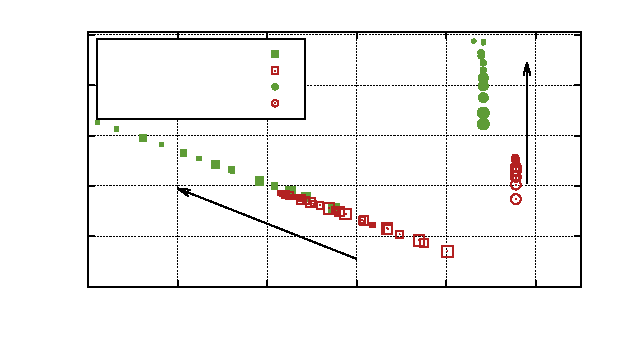
\includegraphics{ConfigurationLowHighRev}}%
    \gplfronttext
  \end{picture}%
\endgroup
}
\end{center}
\caption{Normalized PU and SU capacities for a low PU traffic scenario ($\lambda_{p}=0.1$). Larger points denote higher $k$ values.}\label{BR_fig_LowTraffic}
\end{figure}

Figure \ref{BR_fig_LowTraffic} shows the joint SU-PU performance for the low PU traffic scenario.
Squares correspond to no BR (NBR), and circles to BR performance values. Red and green points correspond to $n_{s,\text{max}}=$ 3 and 6, respectively. 
Larger point sizes indicate larger $k$.
Increasing $\Delta$ allows the discovery of more spectrum opportunities, implying more SU capacity, but less PU capacity (especially without BR) due to a higher collision probability. 
The protection parameter $k$ causes the opposite effect: higher $k$ increases the protection level to PUs (higher $\overline{R}^{\text{nbr}}_{PU}$) and reduces $\overline{R}^{\text{nbr}}_{SU}$. In consequence, the best PU performance, when no BR is used, is attained when $\Delta=n_{s,\text{max}}+k$.
When BR is used, it can be seen that, for each $n_{s,\text{max}}$, all the $\overline{R}^{\text{br}}_{PU}$ values are higher than $\overline{R}^{\text{nbr}}_{PU}$.
\begin{figure}
\begin{center}
\resizebox{9cm}{!}{% GNUPLOT: LaTeX picture with Postscript
\begingroup
  \fontfamily{ptm}%
  \scriptsize
  \selectfont
  \makeatletter
  \providecommand\color[2][]{%
    \GenericError{(gnuplot) \space\space\space\@spaces}{%
      Package color not loaded in conjunction with
      terminal option `colourtext'%
    }{See the gnuplot documentation for explanation.%
    }{Either use 'blacktext' in gnuplot or load the package
      color.sty in LaTeX.}%
    \renewcommand\color[2][]{}%
  }%
  \providecommand\includegraphics[2][]{%
    \GenericError{(gnuplot) \space\space\space\@spaces}{%
      Package graphicx or graphics not loaded%
    }{See the gnuplot documentation for explanation.%
    }{The gnuplot epslatex terminal needs graphicx.sty or graphics.sty.}%
    \renewcommand\includegraphics[2][]{}%
  }%
  \providecommand\rotatebox[2]{#2}%
  \@ifundefined{ifGPcolor}{%
    \newif\ifGPcolor
    \GPcolorfalse
  }{}%
  \@ifundefined{ifGPblacktext}{%
    \newif\ifGPblacktext
    \GPblacktexttrue
  }{}%
  % define a \g@addto@macro without @ in the name:
  \let\gplgaddtomacro\g@addto@macro
  % define empty templates for all commands taking text:
  \gdef\gplbacktext{}%
  \gdef\gplfronttext{}%
  \makeatother
  \ifGPblacktext
    % no textcolor at all
    \def\colorrgb#1{}%
    \def\colorgray#1{}%
  \else
    % gray or color?
    \ifGPcolor
      \def\colorrgb#1{\color[rgb]{#1}}%
      \def\colorgray#1{\color[gray]{#1}}%
      \expandafter\def\csname LTw\endcsname{\color{white}}%
      \expandafter\def\csname LTb\endcsname{\color{black}}%
      \expandafter\def\csname LTa\endcsname{\color{black}}%
      \expandafter\def\csname LT0\endcsname{\color[rgb]{1,0,0}}%
      \expandafter\def\csname LT1\endcsname{\color[rgb]{0,1,0}}%
      \expandafter\def\csname LT2\endcsname{\color[rgb]{0,0,1}}%
      \expandafter\def\csname LT3\endcsname{\color[rgb]{1,0,1}}%
      \expandafter\def\csname LT4\endcsname{\color[rgb]{0,1,1}}%
      \expandafter\def\csname LT5\endcsname{\color[rgb]{1,1,0}}%
      \expandafter\def\csname LT6\endcsname{\color[rgb]{0,0,0}}%
      \expandafter\def\csname LT7\endcsname{\color[rgb]{1,0.3,0}}%
      \expandafter\def\csname LT8\endcsname{\color[rgb]{0.5,0.5,0.5}}%
    \else
      % gray
      \def\colorrgb#1{\color{black}}%
      \def\colorgray#1{\color[gray]{#1}}%
      \expandafter\def\csname LTw\endcsname{\color{white}}%
      \expandafter\def\csname LTb\endcsname{\color{black}}%
      \expandafter\def\csname LTa\endcsname{\color{black}}%
      \expandafter\def\csname LT0\endcsname{\color{black}}%
      \expandafter\def\csname LT1\endcsname{\color{black}}%
      \expandafter\def\csname LT2\endcsname{\color{black}}%
      \expandafter\def\csname LT3\endcsname{\color{black}}%
      \expandafter\def\csname LT4\endcsname{\color{black}}%
      \expandafter\def\csname LT5\endcsname{\color{black}}%
      \expandafter\def\csname LT6\endcsname{\color{black}}%
      \expandafter\def\csname LT7\endcsname{\color{black}}%
      \expandafter\def\csname LT8\endcsname{\color{black}}%
    \fi
  \fi
  \setlength{\unitlength}{0.0500bp}%
  \begin{picture}(5668.00,3571.20)%
    \gplgaddtomacro\gplbacktext{%
      \csname LTb\endcsname%
      \put(602,448){\makebox(0,0)[r]{\strut{} 0}}%
      \csname LTb\endcsname%
      \put(602,886){\makebox(0,0)[r]{\strut{} 0.2}}%
      \csname LTb\endcsname%
      \put(602,1323){\makebox(0,0)[r]{\strut{} 0.4}}%
      \csname LTb\endcsname%
      \put(602,1761){\makebox(0,0)[r]{\strut{} 0.6}}%
      \csname LTb\endcsname%
      \put(602,2199){\makebox(0,0)[r]{\strut{} 0.8}}%
      \csname LTb\endcsname%
      \put(602,2636){\makebox(0,0)[r]{\strut{} 1}}%
      \csname LTb\endcsname%
      \put(602,3074){\makebox(0,0)[r]{\strut{} 1.2}}%
      \csname LTb\endcsname%
      \put(686,308){\makebox(0,0){\strut{}-160}}%
      \csname LTb\endcsname%
      \put(1277,308){\makebox(0,0){\strut{}-140}}%
      \csname LTb\endcsname%
      \put(1868,308){\makebox(0,0){\strut{}-120}}%
      \csname LTb\endcsname%
      \put(2459,308){\makebox(0,0){\strut{}-100}}%
      \csname LTb\endcsname%
      \put(3050,308){\makebox(0,0){\strut{}-80}}%
      \csname LTb\endcsname%
      \put(3642,308){\makebox(0,0){\strut{}-60}}%
      \csname LTb\endcsname%
      \put(4233,308){\makebox(0,0){\strut{}-40}}%
      \csname LTb\endcsname%
      \put(4824,308){\makebox(0,0){\strut{}-20}}%
      \csname LTb\endcsname%
      \put(5415,308){\makebox(0,0){\strut{} 0}}%
      \put(112,1925){\rotatebox{-270}{\makebox(0,0){\strut{}SU Capacity ($\overline{R}^{\text{nbr}}_{SU}$, $\overline{R}^{\text{br}}_{SU}$)}}}%
      \put(3050,98){\makebox(0,0){\strut{}Interference Power ($\overline{R}^{\text{nbr}}_{I}$, $\overline{R}^{\text{br}}_{I}$ in dBm)}}%
      \put(1070,776){\makebox(0,0)[l]{\strut{}$\bar{R}^{\text{br}}_{c}=3.9\cdot 10^{-15}$}}%
      \put(2607,995){\makebox(0,0)[l]{\strut{}$\bar{R}^{\text{br}}_{c}=3.7\cdot10^{-3}$}}%
      \put(3169,667){\makebox(0,0)[l]{\strut{}$\bar{R}^{\text{nbr}}_{c}=3.3\cdot10^{-2}$}}%
      \put(4351,2592){\makebox(0,0)[l]{\strut{}$\bar{R}^{\text{nbr}}_{c}=0.17$}}%
    }%
    \gplgaddtomacro\gplfronttext{%
      \csname LTb\endcsname%
      \put(2198,3226){\makebox(0,0)[r]{\strut{}NBR $n_{s,\text{max}}=6$}}%
      \csname LTb\endcsname%
      \put(2198,3069){\makebox(0,0)[r]{\strut{}NBR $n_{s,\text{max}}=3$}}%
      \csname LTb\endcsname%
      \put(2198,2912){\makebox(0,0)[r]{\strut{}BR $n_{s,\text{max}}=6$}}%
      \csname LTb\endcsname%
      \put(2198,2755){\makebox(0,0)[r]{\strut{}BR $n_{s,\text{max}}=3$}}%
    }%
    \gplbacktext
    \put(0,0){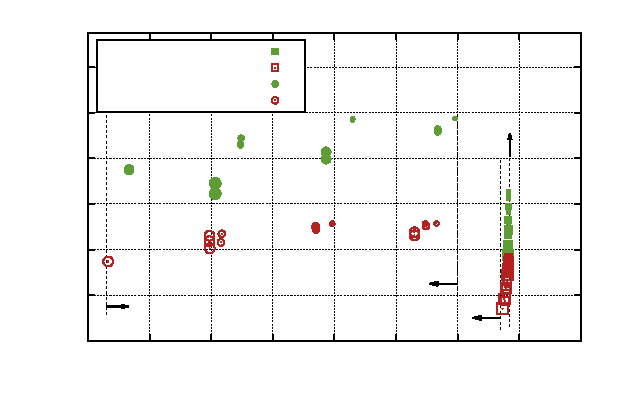
\includegraphics{InterferenceLowHighRev}}%
    \gplfronttext
  \end{picture}%
\endgroup
}
\end{center}
\caption{SU capacity versus interference caused to the PUs for low PU traffic. Larger points denote higher $k$ values. Collision probabilities at the extreme points are indicated.}\label{BR_fig_Interference}
\end{figure}
Figure \ref{BR_fig_Interference}, showing the average interference at the PUs vs. SU capacity, illustrates the reason of the differences between using BR or not: the superior performance of BR in terms of collision/interference, which compensates the negative effect of having fewer channels to allocate at the AN.
However, although BR always manages to reduce collision/interference, it is not always enough to compensate the drawbacks of BR in terms of PU achievable rate. In particular, when the PU traffic is high, there are values of $\overline{R}^{\text{nbr}}_{PU}$ than cannot be achieved with BR, as can be seen in Figure \ref{BR_fig_HighTraffic}. Note, however, that the PU capacity varies in a very short range. Nevertheless, Figure \ref{BR_fig_InterferenceHigh} shows that BR also reduces the interference in the high traffic regime.

\begin{figure}
\begin{center}
\resizebox{9cm}{!}{% GNUPLOT: LaTeX picture with Postscript
\begingroup
  \fontfamily{ptm}%
  \selectfont
  \makeatletter
  \providecommand\color[2][]{%
    \GenericError{(gnuplot) \space\space\space\@spaces}{%
      Package color not loaded in conjunction with
      terminal option `colourtext'%
    }{See the gnuplot documentation for explanation.%
    }{Either use 'blacktext' in gnuplot or load the package
      color.sty in LaTeX.}%
    \renewcommand\color[2][]{}%
  }%
  \providecommand\includegraphics[2][]{%
    \GenericError{(gnuplot) \space\space\space\@spaces}{%
      Package graphicx or graphics not loaded%
    }{See the gnuplot documentation for explanation.%
    }{The gnuplot epslatex terminal needs graphicx.sty or graphics.sty.}%
    \renewcommand\includegraphics[2][]{}%
  }%
  \providecommand\rotatebox[2]{#2}%
  \@ifundefined{ifGPcolor}{%
    \newif\ifGPcolor
    \GPcolorfalse
  }{}%
  \@ifundefined{ifGPblacktext}{%
    \newif\ifGPblacktext
    \GPblacktexttrue
  }{}%
  % define a \g@addto@macro without @ in the name:
  \let\gplgaddtomacro\g@addto@macro
  % define empty templates for all commands taking text:
  \gdef\gplbacktext{}%
  \gdef\gplfronttext{}%
  \makeatother
  \ifGPblacktext
    % no textcolor at all
    \def\colorrgb#1{}%
    \def\colorgray#1{}%
  \else
    % gray or color?
    \ifGPcolor
      \def\colorrgb#1{\color[rgb]{#1}}%
      \def\colorgray#1{\color[gray]{#1}}%
      \expandafter\def\csname LTw\endcsname{\color{white}}%
      \expandafter\def\csname LTb\endcsname{\color{black}}%
      \expandafter\def\csname LTa\endcsname{\color{black}}%
      \expandafter\def\csname LT0\endcsname{\color[rgb]{1,0,0}}%
      \expandafter\def\csname LT1\endcsname{\color[rgb]{0,1,0}}%
      \expandafter\def\csname LT2\endcsname{\color[rgb]{0,0,1}}%
      \expandafter\def\csname LT3\endcsname{\color[rgb]{1,0,1}}%
      \expandafter\def\csname LT4\endcsname{\color[rgb]{0,1,1}}%
      \expandafter\def\csname LT5\endcsname{\color[rgb]{1,1,0}}%
      \expandafter\def\csname LT6\endcsname{\color[rgb]{0,0,0}}%
      \expandafter\def\csname LT7\endcsname{\color[rgb]{1,0.3,0}}%
      \expandafter\def\csname LT8\endcsname{\color[rgb]{0.5,0.5,0.5}}%
    \else
      % gray
      \def\colorrgb#1{\color{black}}%
      \def\colorgray#1{\color[gray]{#1}}%
      \expandafter\def\csname LTw\endcsname{\color{white}}%
      \expandafter\def\csname LTb\endcsname{\color{black}}%
      \expandafter\def\csname LTa\endcsname{\color{black}}%
      \expandafter\def\csname LT0\endcsname{\color{black}}%
      \expandafter\def\csname LT1\endcsname{\color{black}}%
      \expandafter\def\csname LT2\endcsname{\color{black}}%
      \expandafter\def\csname LT3\endcsname{\color{black}}%
      \expandafter\def\csname LT4\endcsname{\color{black}}%
      \expandafter\def\csname LT5\endcsname{\color{black}}%
      \expandafter\def\csname LT6\endcsname{\color{black}}%
      \expandafter\def\csname LT7\endcsname{\color{black}}%
      \expandafter\def\csname LT8\endcsname{\color{black}}%
    \fi
  \fi
  \setlength{\unitlength}{0.0500bp}%
  \begin{picture}(5668.00,3060.00)%
    \gplgaddtomacro\gplbacktext{%
      \csname LTb\endcsname%
      \put(686,705){\makebox(0,0)[r]{\strut{} 0}}%
      \csname LTb\endcsname%
      \put(686,1219){\makebox(0,0)[r]{\strut{} 0.04}}%
      \csname LTb\endcsname%
      \put(686,1734){\makebox(0,0)[r]{\strut{} 0.08}}%
      \csname LTb\endcsname%
      \put(686,2248){\makebox(0,0)[r]{\strut{} 0.12}}%
      \csname LTb\endcsname%
      \put(686,2762){\makebox(0,0)[r]{\strut{} 0.16}}%
      \csname LTb\endcsname%
      \put(770,308){\makebox(0,0){\strut{} 0.988}}%
      \csname LTb\endcsname%
      \put(1434,308){\makebox(0,0){\strut{} 0.99}}%
      \csname LTb\endcsname%
      \put(2097,308){\makebox(0,0){\strut{} 0.992}}%
      \csname LTb\endcsname%
      \put(2761,308){\makebox(0,0){\strut{} 0.994}}%
      \csname LTb\endcsname%
      \put(3424,308){\makebox(0,0){\strut{} 0.996}}%
      \csname LTb\endcsname%
      \put(4088,308){\makebox(0,0){\strut{} 0.998}}%
      \csname LTb\endcsname%
      \put(4751,308){\makebox(0,0){\strut{} 1}}%
      \put(112,1669){\rotatebox{-270}{\makebox(0,0){\strut{}SU Capacity ($\overline{R}^{\text{nbr}}_{SU}$, $\overline{R}^{\text{br}}_{SU}$)}}}%
      \put(3092,98){\makebox(0,0){\strut{}PU Capacity ($\overline{R}^{\text{nbr}}_{PU}$, $\overline{R}^{\text{br}}_{PU}$)}}%
    }%
    \gplgaddtomacro\gplfronttext{%
      \csname LTb\endcsname%
      \put(2282,2680){\makebox(0,0)[r]{\strut{}NBR $n_{s,\text{max}}=6$}}%
      \csname LTb\endcsname%
      \put(2282,2523){\makebox(0,0)[r]{\strut{}NBR $n_{s,\text{max}}=3$}}%
      \csname LTb\endcsname%
      \put(2282,2366){\makebox(0,0)[r]{\strut{}BR $n_{s,\text{max}}=6$}}%
      \csname LTb\endcsname%
      \put(2282,2209){\makebox(0,0)[r]{\strut{}BR $n_{s,\text{max}}=3$}}%
    }%
    \gplbacktext
    \put(0,0){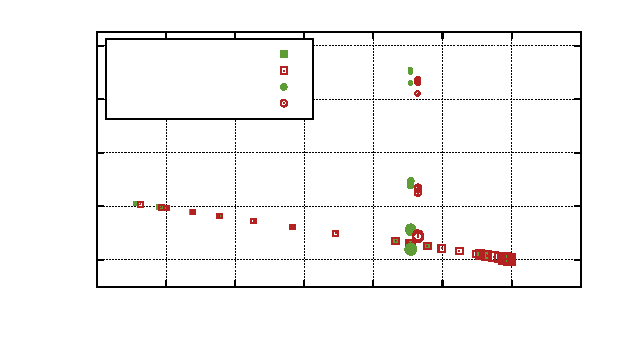
\includegraphics{ConfigurationHighHighRev}}%
    \gplfronttext
  \end{picture}%
\endgroup
}
\end{center}
\caption{SU and PU capacities for a high PU traffic scenario ($\lambda_{p}=0.5$). Larger points denote higher $k$ values.}\label{BR_fig_HighTraffic}
\end{figure}

\begin{figure}
\begin{center}
\resizebox{9cm}{!}{% GNUPLOT: LaTeX picture with Postscript
\begingroup
  \fontfamily{ptm}%
  \scriptsize
  \selectfont
  \makeatletter
  \providecommand\color[2][]{%
    \GenericError{(gnuplot) \space\space\space\@spaces}{%
      Package color not loaded in conjunction with
      terminal option `colourtext'%
    }{See the gnuplot documentation for explanation.%
    }{Either use 'blacktext' in gnuplot or load the package
      color.sty in LaTeX.}%
    \renewcommand\color[2][]{}%
  }%
  \providecommand\includegraphics[2][]{%
    \GenericError{(gnuplot) \space\space\space\@spaces}{%
      Package graphicx or graphics not loaded%
    }{See the gnuplot documentation for explanation.%
    }{The gnuplot epslatex terminal needs graphicx.sty or graphics.sty.}%
    \renewcommand\includegraphics[2][]{}%
  }%
  \providecommand\rotatebox[2]{#2}%
  \@ifundefined{ifGPcolor}{%
    \newif\ifGPcolor
    \GPcolorfalse
  }{}%
  \@ifundefined{ifGPblacktext}{%
    \newif\ifGPblacktext
    \GPblacktexttrue
  }{}%
  % define a \g@addto@macro without @ in the name:
  \let\gplgaddtomacro\g@addto@macro
  % define empty templates for all commands taking text:
  \gdef\gplbacktext{}%
  \gdef\gplfronttext{}%
  \makeatother
  \ifGPblacktext
    % no textcolor at all
    \def\colorrgb#1{}%
    \def\colorgray#1{}%
  \else
    % gray or color?
    \ifGPcolor
      \def\colorrgb#1{\color[rgb]{#1}}%
      \def\colorgray#1{\color[gray]{#1}}%
      \expandafter\def\csname LTw\endcsname{\color{white}}%
      \expandafter\def\csname LTb\endcsname{\color{black}}%
      \expandafter\def\csname LTa\endcsname{\color{black}}%
      \expandafter\def\csname LT0\endcsname{\color[rgb]{1,0,0}}%
      \expandafter\def\csname LT1\endcsname{\color[rgb]{0,1,0}}%
      \expandafter\def\csname LT2\endcsname{\color[rgb]{0,0,1}}%
      \expandafter\def\csname LT3\endcsname{\color[rgb]{1,0,1}}%
      \expandafter\def\csname LT4\endcsname{\color[rgb]{0,1,1}}%
      \expandafter\def\csname LT5\endcsname{\color[rgb]{1,1,0}}%
      \expandafter\def\csname LT6\endcsname{\color[rgb]{0,0,0}}%
      \expandafter\def\csname LT7\endcsname{\color[rgb]{1,0.3,0}}%
      \expandafter\def\csname LT8\endcsname{\color[rgb]{0.5,0.5,0.5}}%
    \else
      % gray
      \def\colorrgb#1{\color{black}}%
      \def\colorgray#1{\color[gray]{#1}}%
      \expandafter\def\csname LTw\endcsname{\color{white}}%
      \expandafter\def\csname LTb\endcsname{\color{black}}%
      \expandafter\def\csname LTa\endcsname{\color{black}}%
      \expandafter\def\csname LT0\endcsname{\color{black}}%
      \expandafter\def\csname LT1\endcsname{\color{black}}%
      \expandafter\def\csname LT2\endcsname{\color{black}}%
      \expandafter\def\csname LT3\endcsname{\color{black}}%
      \expandafter\def\csname LT4\endcsname{\color{black}}%
      \expandafter\def\csname LT5\endcsname{\color{black}}%
      \expandafter\def\csname LT6\endcsname{\color{black}}%
      \expandafter\def\csname LT7\endcsname{\color{black}}%
      \expandafter\def\csname LT8\endcsname{\color{black}}%
    \fi
  \fi
  \setlength{\unitlength}{0.0500bp}%
  \begin{picture}(5668.00,3060.00)%
    \gplgaddtomacro\gplbacktext{%
      \csname LTb\endcsname%
      \put(686,705){\makebox(0,0)[r]{\strut{} 0}}%
      \csname LTb\endcsname%
      \put(686,1219){\makebox(0,0)[r]{\strut{} 0.04}}%
      \csname LTb\endcsname%
      \put(686,1734){\makebox(0,0)[r]{\strut{} 0.08}}%
      \csname LTb\endcsname%
      \put(686,2248){\makebox(0,0)[r]{\strut{} 0.12}}%
      \csname LTb\endcsname%
      \put(686,2762){\makebox(0,0)[r]{\strut{} 0.16}}%
      \csname LTb\endcsname%
      \put(770,308){\makebox(0,0){\strut{}-160}}%
      \csname LTb\endcsname%
      \put(1351,308){\makebox(0,0){\strut{}-140}}%
      \csname LTb\endcsname%
      \put(1931,308){\makebox(0,0){\strut{}-120}}%
      \csname LTb\endcsname%
      \put(2512,308){\makebox(0,0){\strut{}-100}}%
      \csname LTb\endcsname%
      \put(3093,308){\makebox(0,0){\strut{}-80}}%
      \csname LTb\endcsname%
      \put(3673,308){\makebox(0,0){\strut{}-60}}%
      \csname LTb\endcsname%
      \put(4254,308){\makebox(0,0){\strut{}-40}}%
      \csname LTb\endcsname%
      \put(4834,308){\makebox(0,0){\strut{}-20}}%
      \csname LTb\endcsname%
      \put(5415,308){\makebox(0,0){\strut{} 0}}%
      \put(112,1669){\rotatebox{-270}{\makebox(0,0){\strut{}SU Capacity ($\overline{R}^{\text{nbr}}_{SU}$, $\overline{R}^{\text{br}}_{SU}$)}}}%
      \put(3092,98){\makebox(0,0){\strut{}Interference Power ($\overline{R}^{\text{nbr}}_{I}$, $\overline{R}^{\text{br}}_{I}$ in dBm)}}%
    }%
    \gplgaddtomacro\gplfronttext{%
      \csname LTb\endcsname%
      \put(2282,2680){\makebox(0,0)[r]{\strut{}NBR $n_{s,\text{max}}=6$}}%
      \csname LTb\endcsname%
      \put(2282,2523){\makebox(0,0)[r]{\strut{}NBR $n_{s,\text{max}}=3$}}%
      \csname LTb\endcsname%
      \put(2282,2366){\makebox(0,0)[r]{\strut{}BR $n_{s,\text{max}}=6$}}%
      \csname LTb\endcsname%
      \put(2282,2209){\makebox(0,0)[r]{\strut{}BR $n_{s,\text{max}}=3$}}%
    }%
    \gplbacktext
    \put(0,0){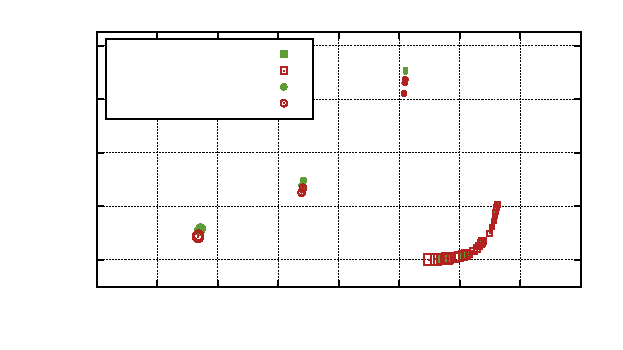
\includegraphics{InterferenceHighHighRev}}%
    \gplfronttext
  \end{picture}%
\endgroup
}
\end{center}
\caption{SU capacity versus interference caused to the PUs for high PU traffic.}\label{BR_fig_InterferenceHigh}
\end{figure}

\subsection{Studying PU motivation to use BR}
We have seen that the PU traffic intensity is closely related to the performance limits on $\overline{R}^{\text{br}}_{PU}$. This suggests that an AN implementing BR could decide to switch this feature on or off, depending on its own traffic load. To see where the traffic threshold could be located, we represent, in Figure \ref{BR_fig_Thresholds}, the highest values of $\overline{R}^{\text{br}}_{PU}$ and $\overline{R}^{\text{nbr}}_{PU}$ for $n_{s,\text{max}}=4$. To assess the effect of SU traffic as well, several $\rho_{s}$ values are used (0.1,0.5,0.8). It can be seen that, without BR, the PU capacity is higher for larger $\lambda_{p}$, because the spectrum sensing detects more PU activity and incoming SUs either do not transmit or transmit using very few channels, reducing the effects of interference/collision.
\begin{figure}[ht]
\begin{center}
\resizebox{9cm}{!}{% GNUPLOT: LaTeX picture with Postscript
\begingroup
  \fontfamily{ptm}%
  \scriptsize 
  \selectfont
  \makeatletter
  \providecommand\color[2][]{%
    \GenericError{(gnuplot) \space\space\space\@spaces}{%
      Package color not loaded in conjunction with
      terminal option `colourtext'%
    }{See the gnuplot documentation for explanation.%
    }{Either use 'blacktext' in gnuplot or load the package
      color.sty in LaTeX.}%
    \renewcommand\color[2][]{}%
  }%
  \providecommand\includegraphics[2][]{%
    \GenericError{(gnuplot) \space\space\space\@spaces}{%
      Package graphicx or graphics not loaded%
    }{See the gnuplot documentation for explanation.%
    }{The gnuplot epslatex terminal needs graphicx.sty or graphics.sty.}%
    \renewcommand\includegraphics[2][]{}%
  }%
  \providecommand\rotatebox[2]{#2}%
  \@ifundefined{ifGPcolor}{%
    \newif\ifGPcolor
    \GPcolorfalse
  }{}%
  \@ifundefined{ifGPblacktext}{%
    \newif\ifGPblacktext
    \GPblacktexttrue
  }{}%
  % define a \g@addto@macro without @ in the name:
  \let\gplgaddtomacro\g@addto@macro
  % define empty templates for all commands taking text:
  \gdef\gplbacktext{}%
  \gdef\gplfronttext{}%
  \makeatother
  \ifGPblacktext
    % no textcolor at all
    \def\colorrgb#1{}%
    \def\colorgray#1{}%
  \else
    % gray or color?
    \ifGPcolor
      \def\colorrgb#1{\color[rgb]{#1}}%
      \def\colorgray#1{\color[gray]{#1}}%
      \expandafter\def\csname LTw\endcsname{\color{white}}%
      \expandafter\def\csname LTb\endcsname{\color{black}}%
      \expandafter\def\csname LTa\endcsname{\color{black}}%
      \expandafter\def\csname LT0\endcsname{\color[rgb]{1,0,0}}%
      \expandafter\def\csname LT1\endcsname{\color[rgb]{0,1,0}}%
      \expandafter\def\csname LT2\endcsname{\color[rgb]{0,0,1}}%
      \expandafter\def\csname LT3\endcsname{\color[rgb]{1,0,1}}%
      \expandafter\def\csname LT4\endcsname{\color[rgb]{0,1,1}}%
      \expandafter\def\csname LT5\endcsname{\color[rgb]{1,1,0}}%
      \expandafter\def\csname LT6\endcsname{\color[rgb]{0,0,0}}%
      \expandafter\def\csname LT7\endcsname{\color[rgb]{1,0.3,0}}%
      \expandafter\def\csname LT8\endcsname{\color[rgb]{0.5,0.5,0.5}}%
    \else
      % gray
      \def\colorrgb#1{\color{black}}%
      \def\colorgray#1{\color[gray]{#1}}%
      \expandafter\def\csname LTw\endcsname{\color{white}}%
      \expandafter\def\csname LTb\endcsname{\color{black}}%
      \expandafter\def\csname LTa\endcsname{\color{black}}%
      \expandafter\def\csname LT0\endcsname{\color{black}}%
      \expandafter\def\csname LT1\endcsname{\color{black}}%
      \expandafter\def\csname LT2\endcsname{\color{black}}%
      \expandafter\def\csname LT3\endcsname{\color{black}}%
      \expandafter\def\csname LT4\endcsname{\color{black}}%
      \expandafter\def\csname LT5\endcsname{\color{black}}%
      \expandafter\def\csname LT6\endcsname{\color{black}}%
      \expandafter\def\csname LT7\endcsname{\color{black}}%
      \expandafter\def\csname LT8\endcsname{\color{black}}%
    \fi
  \fi
  \setlength{\unitlength}{0.0500bp}%
  \begin{picture}(5668.00,3968.00)%
    \gplgaddtomacro\gplbacktext{%
      \csname LTb\endcsname%
      \put(686,448){\makebox(0,0)[r]{\strut{} 0.9}}%
      \csname LTb\endcsname%
      \put(686,1057){\makebox(0,0)[r]{\strut{} 0.92}}%
      \csname LTb\endcsname%
      \put(686,1667){\makebox(0,0)[r]{\strut{} 0.94}}%
      \csname LTb\endcsname%
      \put(686,2276){\makebox(0,0)[r]{\strut{} 0.96}}%
      \csname LTb\endcsname%
      \put(686,2885){\makebox(0,0)[r]{\strut{} 0.98}}%
      \csname LTb\endcsname%
      \put(686,3494){\makebox(0,0)[r]{\strut{} 1}}%
      \csname LTb\endcsname%
      \put(770,308){\makebox(0,0){\strut{} 0}}%
      \csname LTb\endcsname%
      \put(1544,308){\makebox(0,0){\strut{} 0.1}}%
      \csname LTb\endcsname%
      \put(2318,308){\makebox(0,0){\strut{} 0.2}}%
      \csname LTb\endcsname%
      \put(3092,308){\makebox(0,0){\strut{} 0.3}}%
      \csname LTb\endcsname%
      \put(3867,308){\makebox(0,0){\strut{} 0.4}}%
      \csname LTb\endcsname%
      \put(4641,308){\makebox(0,0){\strut{} 0.5}}%
      \csname LTb\endcsname%
      \put(5415,308){\makebox(0,0){\strut{} 0.6}}%
      \put(112,2123){\rotatebox{-270}{\makebox(0,0){\strut{}PU Capacity ($\overline{R}^{\text{nbr}}_{PU}$, $\overline{R}^{\text{br}}_{PU}$)}}}%
      \put(3092,98){\makebox(0,0){\strut{}PU Arrival Rate ($\lambda_{p}$)}}%
      \put(1776,905){\makebox(0,0)[l]{\strut{}$\rho_{s} = 0.8$}}%
      \put(1854,1636){\makebox(0,0)[l]{\strut{}$\rho_{s} = 0.5$}}%
      \put(847,2733){\makebox(0,0)[l]{\strut{}$\rho_{s} = 0.1$}}%
      \put(2628,2611){\makebox(0,0)[l]{\strut{}(BR) $\rho_{s} = 0.1,0.5,0.8$}}%
    }%
    \gplgaddtomacro\gplfronttext{%
      \csname LTb\endcsname%
      \put(4764,1131){\makebox(0,0)[r]{\strut{}NBR}}%
      \csname LTb\endcsname%
      \put(4764,974){\makebox(0,0)[r]{\strut{}NBR approx.}}%
      \csname LTb\endcsname%
      \put(4764,817){\makebox(0,0)[r]{\strut{}BR}}%
      \csname LTb\endcsname%
      \put(4764,660){\makebox(0,0)[r]{\strut{}BR approx.}}%
    }%
    \gplbacktext
    \put(0,0){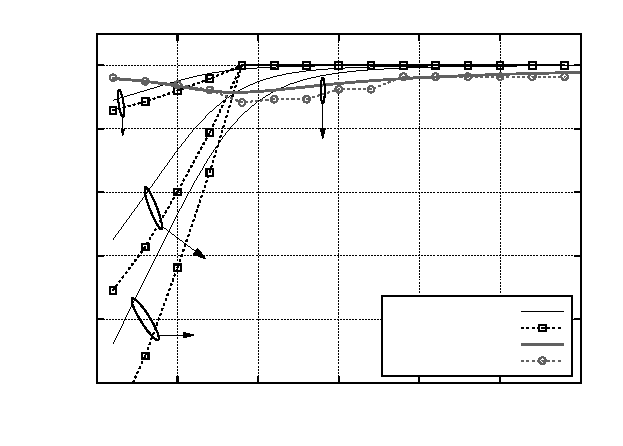
\includegraphics{PUcapacityRev}}%
    \gplfronttext
  \end{picture}%
\endgroup
}
\end{center}
\caption{Effect of PU and SU traffic intensities on PU capacity. Approximate values $\tilde{R}^{\text{nbr}}_{PU}$, $\tilde{R}^{\text{br}}_{PU}$ are represented with points and dotted lines. For each SU traffic intensity there is a PU traffic threshold value below which the PU would prefer to activate BR.}\label{BR_fig_Thresholds}
\end{figure}
We can obtain an estimation of the traffic thresholds without resorting to the Markov model by means of approximate expressions for $\overline{R}^{\text{nbr}}_{PU}$ and $\overline{R}^{\text{br}}_{PU}$. Assuming that the spectrum contains an SU transmission with probability $\rho_{s}$, we can compute the following average:
\begin{equation}
\tilde{R}^{\ast}_{PU} = C^{\ast}_{N}\left(\left\lfloor \tilde{n}_{p}\right\rceil,\left\lfloor \tilde{n}_{s}\right\rceil\right)\rho_{s} + C^{\ast}_{N}\left(\left\lfloor \tilde{n}_{p}\right\rceil\right)\left(1-\rho_{s}\right)
\end{equation}
where $\ast = \text{nbr}$ or $\text{br}$, $\left\lfloor x\right\rceil$ denotes the closest integer to $x$, and $\tilde{n}_{p}$, $\tilde{n}_{s}$ are estimates of the average values of $n_{p}$ and $n_{s}$. We have that $\tilde{n}_{p} = \sum_{i=0}^{N}i\pi_{i}$, and $\tilde{n}_{s} = \sum_{i=0}^{N}\theta_{\ast}(i)\pi_{i}$, where
\begin{equation}
\begin{array}{lcl}
\theta_{\text{nbr}}(n_{p}) & = & \text{min}\left(\frac{N-n_{p}}{N}\Delta-k,n_{s,\text{max}}\right)\\
\theta_{\text{br}}(n_{p}) & = & \text{min}\left(N-n_{p}-k,n_{s,\text{max}}\right)
\end{array}
\end{equation}
and $\frac{N-n_{p}}{N}\Delta$ is the expected number of available channels in $\Delta$. 
The approximate capacity values obtained with this approximation are also shown in Figure \ref{BR_fig_Thresholds}.
Finally, Figure \ref{BR_fig_sim_interference} depicts the interference power at the PU receivers for different PU and SU traffic regimes. When the traffic increases, the BR average interference power converges to the no BR case, because the reserved channels are more frequently used by PU transmissions resulting in higher collision probability.
\begin{figure}[ht]
\begin{center}
\resizebox{9cm}{!}{% GNUPLOT: LaTeX picture with Postscript
\begingroup
  \fontfamily{ptm}%
  \scriptsize
  \selectfont
  \makeatletter
  \providecommand\color[2][]{%
    \GenericError{(gnuplot) \space\space\space\@spaces}{%
      Package color not loaded in conjunction with
      terminal option `colourtext'%
    }{See the gnuplot documentation for explanation.%
    }{Either use 'blacktext' in gnuplot or load the package
      color.sty in LaTeX.}%
    \renewcommand\color[2][]{}%
  }%
  \providecommand\includegraphics[2][]{%
    \GenericError{(gnuplot) \space\space\space\@spaces}{%
      Package graphicx or graphics not loaded%
    }{See the gnuplot documentation for explanation.%
    }{The gnuplot epslatex terminal needs graphicx.sty or graphics.sty.}%
    \renewcommand\includegraphics[2][]{}%
  }%
  \providecommand\rotatebox[2]{#2}%
  \@ifundefined{ifGPcolor}{%
    \newif\ifGPcolor
    \GPcolorfalse
  }{}%
  \@ifundefined{ifGPblacktext}{%
    \newif\ifGPblacktext
    \GPblacktexttrue
  }{}%
  % define a \g@addto@macro without @ in the name:
  \let\gplgaddtomacro\g@addto@macro
  % define empty templates for all commands taking text:
  \gdef\gplbacktext{}%
  \gdef\gplfronttext{}%
  \makeatother
  \ifGPblacktext
    % no textcolor at all
    \def\colorrgb#1{}%
    \def\colorgray#1{}%
  \else
    % gray or color?
    \ifGPcolor
      \def\colorrgb#1{\color[rgb]{#1}}%
      \def\colorgray#1{\color[gray]{#1}}%
      \expandafter\def\csname LTw\endcsname{\color{white}}%
      \expandafter\def\csname LTb\endcsname{\color{black}}%
      \expandafter\def\csname LTa\endcsname{\color{black}}%
      \expandafter\def\csname LT0\endcsname{\color[rgb]{1,0,0}}%
      \expandafter\def\csname LT1\endcsname{\color[rgb]{0,1,0}}%
      \expandafter\def\csname LT2\endcsname{\color[rgb]{0,0,1}}%
      \expandafter\def\csname LT3\endcsname{\color[rgb]{1,0,1}}%
      \expandafter\def\csname LT4\endcsname{\color[rgb]{0,1,1}}%
      \expandafter\def\csname LT5\endcsname{\color[rgb]{1,1,0}}%
      \expandafter\def\csname LT6\endcsname{\color[rgb]{0,0,0}}%
      \expandafter\def\csname LT7\endcsname{\color[rgb]{1,0.3,0}}%
      \expandafter\def\csname LT8\endcsname{\color[rgb]{0.5,0.5,0.5}}%
    \else
      % gray
      \def\colorrgb#1{\color{black}}%
      \def\colorgray#1{\color[gray]{#1}}%
      \expandafter\def\csname LTw\endcsname{\color{white}}%
      \expandafter\def\csname LTb\endcsname{\color{black}}%
      \expandafter\def\csname LTa\endcsname{\color{black}}%
      \expandafter\def\csname LT0\endcsname{\color{black}}%
      \expandafter\def\csname LT1\endcsname{\color{black}}%
      \expandafter\def\csname LT2\endcsname{\color{black}}%
      \expandafter\def\csname LT3\endcsname{\color{black}}%
      \expandafter\def\csname LT4\endcsname{\color{black}}%
      \expandafter\def\csname LT5\endcsname{\color{black}}%
      \expandafter\def\csname LT6\endcsname{\color{black}}%
      \expandafter\def\csname LT7\endcsname{\color{black}}%
      \expandafter\def\csname LT8\endcsname{\color{black}}%
    \fi
  \fi
  \setlength{\unitlength}{0.0500bp}%
  \begin{picture}(5668.00,3400.00)%
    \gplgaddtomacro\gplbacktext{%
      \csname LTb\endcsname%
      \put(602,448){\makebox(0,0)[r]{\strut{}-120}}%
      \csname LTb\endcsname%
      \put(602,1005){\makebox(0,0)[r]{\strut{}-100}}%
      \csname LTb\endcsname%
      \put(602,1561){\makebox(0,0)[r]{\strut{}-80}}%
      \csname LTb\endcsname%
      \put(602,2118){\makebox(0,0)[r]{\strut{}-60}}%
      \csname LTb\endcsname%
      \put(602,2674){\makebox(0,0)[r]{\strut{}-40}}%
      \csname LTb\endcsname%
      \put(602,3231){\makebox(0,0)[r]{\strut{}-20}}%
      \csname LTb\endcsname%
      \put(686,308){\makebox(0,0){\strut{} 0}}%
      \csname LTb\endcsname%
      \put(1474,308){\makebox(0,0){\strut{} 0.1}}%
      \csname LTb\endcsname%
      \put(2262,308){\makebox(0,0){\strut{} 0.2}}%
      \csname LTb\endcsname%
      \put(3050,308){\makebox(0,0){\strut{} 0.3}}%
      \csname LTb\endcsname%
      \put(3839,308){\makebox(0,0){\strut{} 0.4}}%
      \csname LTb\endcsname%
      \put(4627,308){\makebox(0,0){\strut{} 0.5}}%
      \csname LTb\endcsname%
      \put(5415,308){\makebox(0,0){\strut{} 0.6}}%
      \put(112,1839){\rotatebox{-270}{\makebox(0,0){\strut{}Interference Power (dBm)}}}%
      \put(3050,98){\makebox(0,0){\strut{}PU Arrival Rate ($\lambda_{p}$)}}%
      \put(1671,2340){\makebox(0,0)[l]{\strut{}NBR}}%
      \put(1829,1255){\makebox(0,0)[l]{\strut{}BR}}%
    }%
    \gplgaddtomacro\gplfronttext{%
      \csname LTb\endcsname%
      \put(4764,1445){\makebox(0,0)[r]{\strut{}NBR $\rho_{s}=0.1$}}%
      \csname LTb\endcsname%
      \put(4764,1288){\makebox(0,0)[r]{\strut{}NBR $\rho_{s}=0.5$}}%
      \csname LTb\endcsname%
      \put(4764,1131){\makebox(0,0)[r]{\strut{}NBR $\rho_{s}=0.8$}}%
      \csname LTb\endcsname%
      \put(4764,974){\makebox(0,0)[r]{\strut{}BR $\rho_{s}=0.1$}}%
      \csname LTb\endcsname%
      \put(4764,817){\makebox(0,0)[r]{\strut{}BR $\rho_{s}=0.5$}}%
      \csname LTb\endcsname%
      \put(4764,660){\makebox(0,0)[r]{\strut{}BR $\rho_{s}=0.8$}}%
    }%
    \gplbacktext
    \put(0,0){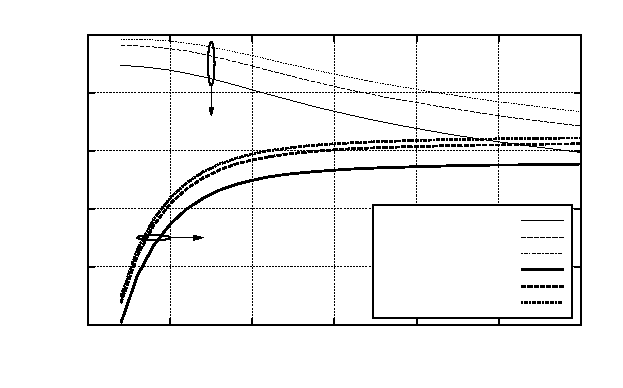
\includegraphics{PUinterferenceRev}}%
    \gplfronttext
  \end{picture}%
\endgroup
}
\end{center}
\caption{Effect of PU and SU traffic intensities on the interference at PUs.}\label{BR_fig_sim_interference}
\end{figure}

\section{Conclusions}\label{sec:Conclusion}
Even with the sensing capabilities of cognitive radios, OSA is always associated to some degree of transmission overlapping with PU transmissions and therefore to harmful interference at PU receivers. 
This chapter studies the idea of a primary network reserving some part of its spectrum for OSA to reduce harmful interference from SUs. 
The reserved channels are only used for PU transmissions when the rest of the channels overflow.
We have developed a Markov-reward model for evaluating the PU and SU capacities in coexistence scenarios with and without bandwidth reservation.
The numerical results showed that using BR implies moderate PU capacity reduction, e.g. reserving 4 out of 15 channels, resulted in a PU capacity reduction of 1\% in the worst case. If the PU traffic intensity is below a certain value, the PU capacity obtained with BR is higher than the capacity achieved without BR, because of the better interference (and collision probability) performance of BR.  
The AN is therefore motivated to activate BR under low traffic regimes. For the SUs there is a remarkable performance improvement when using the reserved spectrum, resulting in a higher spectrum efficiency.
Our model is applicable to the design of BR activation policies, using either the Markov framework or a simpler approximate formulation.